\documentclass[12pt]{article}
\usepackage{anyfontsize}
\usepackage[a4paper, margin=2cm]{geometry}
\usepackage{polski}
\usepackage{tabto}
\usepackage{enumitem}
\usepackage{amsmath}
\usepackage{amssymb}
\usepackage{multirow}
\usepackage{multicol}
\usepackage{setspace}
\usepackage{listings}
\input{verticalPages.tex}

\setlength{\emergencystretch}{10pt}


\usepackage{tabularx}
\newcolumntype{C}{>{\centering\arraybackslash}X}
\newcolumntype{L}{>{\raggedleft\arraybackslash}X}
\newcolumntype{R}{>{\raggedright\arraybackslash}X}
\newcommand{\centerY}[2]{\multirow{#1}{*}{#2}}

\usepackage{wrapfig}
\usepackage{subcaption}

\usepackage{hyperref}
\hypersetup{
    colorlinks = true,
    urlcolor=blue,
    linkcolor= black,
    citecolor= blue
}

\usepackage{chngcntr}
\counterwithin{figure}{section}
\counterwithin{table}{section}
\numberwithin{equation}{section}

\usepackage{graphicx}
\graphicspath{{./Img/}}

\usepackage{csvsimple}
\usepackage{pgfplots}
\usepackage{pgfplotstable}
\pgfplotsset{compat= newest}


\usepackage{titlesec}
\titlelabel{\thetitle.\quad}
% \AddToHook{cmd/section/before}{\clearpage}

\usepackage[european, american currents, americanvoltages, RPvoltages, cute inductor]{circuitikz}
\usepackage{tikz}
\usetikzlibrary{shapes.geometric}
\ctikzset{
    logic ports=ieee,
    logic ports/scale=0.7,
}


\usepackage[polish]{babel}
\usepackage{csquotes}
\usepackage[sorting=none]{biblatex}
\bibliography{bibliography.bib}

\lstdefinestyle{asm}{
    belowcaptionskip=1\baselineskip,
    frame=L,
    xleftmargin=\parindent,
    showstringspaces=false,
    numbers=left,
    firstnumber=1,
    basicstyle=\footnotesize,
    basicstyle=\ttfamily,
    tabsize=4,
}


\usepackage{listings}
\lstset{
literate=%
    {ą}{{\k{a}}}1
    {Ą}{{\k{A}}}1
    {ć}{{\'c}}1
    {Ć}{{\'{C}}}1
    {ę}{{\k{e}}}1
    {Ę}{{\k{E}}}1
    {ł}{{\l{}}}1
    {Ł}{{\L{}}}1
    {ń}{{\'n}}1
    {Ń}{{\'N}}1
    {ó}{{\'o}}1
    {Ó}{{\'O}}1
    {ś}{{\'s}}1
    {Ś}{{\'S}}1
    {ż}{{\.z}}1
    {Ż}{{\.Z}}1
    {ź}{{\'z}}1
    {Ź}{{\'Z}}1
}


\title{
    \includegraphics[width = 0.3\textwidth]{agh_logo.jpg}\\
    \textbf{Akademia Górniczo-Hutnicza w Krakowie}\\
    Wydział Informatyki, Elektroniki i  Telekomunikacji\\\vspace{2cm}
    \textbf{Praca inżynierska}\\
    Pojazd autonomiczny służący do pokonywania trasy z~przeszkodami\\\vspace{1cm}
    \small{An autonomous vehicle designed to navigate an obstacle course}
}
\author{
    \begin{tabularx}{\textwidth}{l l}
    Autor: &Łukasz Przystupa\\
    Kierunek studiów: & Elektronika\\
    Opiekun pracy: &dr inż. Agnieszka Dąbrowska-Boruch
    \end{tabularx}
}
\date{\vspace{2cm}\today}

\usepackage{titling}
\renewcommand\maketitlehooka{\null\mbox{}\vfill}
\renewcommand\maketitlehookd{\vfill\null}

\begin{document}
    \begin{titlepage}
        \maketitle
        \thispagestyle{empty}
        \newpage
        \
        \thispagestyle{empty}
    \end{titlepage}

    \pagenumbering{Roman}
        \section*{Spis skrótów}
\addcontentsline{toc}{section}{Spis skrótów}
\begin{table*}[!ht]
    \begin{tabularx}{\textwidth}{|c|C|C|}\hline
        Skrót & Rozszerzenie\ & Opis\\\hline
        \centerY{2}{GPIO}       & \centerY{2}{General Purpose Input/Output} & Wyprowadzenia z układów scalonych do dowolnego wykorzystania\\\hline
        \centerY{2}{DIY}        & \centerY{2}{Do It Yourself} & Projekt do własnoręcznego wykonania\\\hline
        \centerY{2}{SSH}        & \centerY{2}{Secure Shell} & Protokół komunikacyjny, pozwalający na bezpieczne połączenie do serwera\\\hline
        \centerY{2}{HAL}        & \centerY{2}{Hardware Abstraction Layer} & Sposób porozumiewania się ze sprzętem\\\hline
        \centerY{3}{PWM}        & \centerY{3}{Pulse Wave Modulation} & Rodzaj modulacji cyfrowych pozwalający na regulację wypełnienia sygnału\\\hline
        \centerY{3}{ToF}        & \centerY{3}{Time of Flight} & Rodzaj czujników pomiaru odległości, polegający na pomiarze czasu przelotu wiązki światła\\\hline
        \centerY{1}{IR}         & \centerY{1}{Infrared} & Czujniki wykrywające promieniowanie podczerwone\\\hline
        \centerY{2}{CAD}        & \centerY{2}{Computer Aided Design} & Zestaw narzędzi do projektowania np.~modeli 3D\\\hline
        \centerY{1}{RB Pi Pico} & \centerY{1}{Raspberry Pi Pico} & Mikrokontroler firmy Raspberry Pi\\\hline
    \end{tabularx}
\end{table*}
        \tableofcontents
        \newpage
    \pagenumbering{arabic}
    % \input{Chapters/Abstract.tex}
    \section{Wstęp}
    Celem poniższej pracy jest skonstruowanie autonomicznego pojazdu, którego zadaniem będzie zbudowanie wirtualnej mapy terenu oraz samodzielne poruszanie się po nieznanym obszarze.
    Jednym z założeń projektu jest umożliwienie użytkownikowi kontroli nad pojazdem za pomocą dedykowanej aplikacji komputerowej.
    Dodatkowo, powyższa aplikacja będzie wyświetlać budowaną mapę w czasie rzeczywistym.
    Po wskazaniu punktu docelowego, zostanie zaproponowana optymalna trasa, po której pojazd będzie się poruszał.


    \subsection{Środowisko sprzętowe}
        Współczesne pojazdy autonomiczne wyposażone są w jednostki obliczeniowe, które swoją konstrukcją przypominają pełnoprawne komputery z systemem operacyjnym.
        Ten projekt ma być modelem,  przedstawiającym działanie pojazdu autonomicznego, dlatego wykorzystanie pełnoprawnego komputera jest zbędne.

        \subsubsection{Mikrokontroler}
            Poniżej przedstawiono kilka najbardziej popularnym platform sprzętowych, które mogą stanowić bazę dla pojazdu.
            \begin{enumerate}
                \item Raspberry Pi -- komputer z systemem operacyjnym Linux, umożliwiający bezpośredni dostęp do modułów zewnętrznych z pomocą GPIO.
                Jest to najbardziej popularna platforma dla projektów DIY.
                Układ pozwala na niesamowitą elastyczność w pracy, między innymi na podłączenie się do układu za pośrednictwem SSH oraz pracę w języku Python.
                Jednak ze względu na swoją popularność, jest bardzo drogi i mało dostępny.
                Natomiast, jednym z założeń projektu jest działanie w czasie rzeczywistym, co przy wykorzystaniu systemu operacyjnego jest niemożliwe.
                \item Arduino -- najpopularniejsza platforma, której głównymi zaletami są: prostota framework'u oraz mnogość bibliotek dla każdego układu.
                Niestety, płytki te oparte są o 8-bitowe mikrokontrolery z rodziny AVR, co odbija się na ich prędkościach  (max 20MHz).
                Sam framework wykorzystywany jest na wielu różnych praformach, przez co w dłuższej perspektywie staje się nieintuicyjny.
                \item STM32 -- układy projektowane przez firmę STMicroelectronics. Są znacznie szybsze i posiadają więcej pamięci od Arduino.
                Jednak ze względu na potrzebę wykorzystania biblioteki HAL, programowanie jest znacznie trudniejsze w porównaniu do innych układów.
                \item ESP32 -- 32-bitowy dwurdzeniowy procesor z wbudowanym modułem WiFi i Bluetooth.
                Jeden z najszybszych mikrokontrolerów dostępnych na rynku. Jest bardzo popularny w projektach IoT (wytłumaczyć).
                Natywnie pracuje w systemie czasu rzeczywistego - FreeRTOS. Dzięki temu ma potencjał na bycie idealnym kandydatem do tego projektu.
                Jednak znikoma dokumentacja produktu sprawia, że praca z nim jest uciążliwa, przez co opracowanie optymalnego kodu jest znacząco utrudnione.
                \item Raspberry Pi Pico -- mikrokontroler od firmy Raspberry Pi, oparty na rdzeniach Cortex - tak samo jak STM32.
                Producent udostępnił wyjątkowo przystępny zestaw narzędzi programistycznych oraz przykładów użycia.
                Kolejną z zalet jest dobra dokumentacja tego procesora, która jest stale rozwijana.
                W 2022 roku, pojawiła się druga iteracja tej płytki Raspberry Pi Pico~W ze zintegrowanym modułem WiFi.
            \end{enumerate}
            Projekt jest możliwy do zrealizowania na wszystkich wymienionych powyżej platformach.
            Jednak ze względu na swoją przystępność, Raspberry Pi Pico jest najbardziej optymalnym wyborem.
            \begin{figure}[!ht]
                \centering
                \includegraphics[width = 0.3\textwidth]{raspberry_pico.png}
                \caption{Raspberry Pi Pico}
                Źródło: \href{https://botland.com.pl/moduly-i-zestawy-do-raspberry-pi-pico/21574-raspberry-pi-pico-w-rp2040-arm-cortex-m0-cyw43439-wifi-5056561803173.html}{botland.com}

                % Źródło: https://botland.com.pl/silniki-dc-z-przekladnia-i-enkoderami/6287-silnik-z-przekladnia-sj01-120-1-6v-160rpm-enkoder-6959420910205.html
                % Źródło: https://botland.com.pl/serwa-typu-micro/20435-serwo-mg-90s-micro-180-stopni-metalowa-przekladnia-5904422380915.html
                \label{fig:raspberry_pico}
            \end{figure}

        \subsubsection{Sterowanie}
        \label{sec:engines}
            Podstawowym zadaniem pojazdów mechanicznych jest poruszanie się.
            Dlatego niezwykle istotne było wybranie odpowiedniego silnika napędowego.
            Na rynku konsumenckim istnieje jest wiele ich wariantów.
            Poniżej opisano możliwe rozwiązania oraz skrótowo omówiono ich wady i zalety:
            \begin{enumerate}
                \item Silniki krokowe -- niegdyś bardzo duże i drogie silniki, wymagające dodatkowych układów sterujących.
                Dziś jednak istnieją mniejsze, niskonapięciowe rozwiązania, które mogą być kontrolowaneZ bezpośrednio przez mikroprocesor.
                Niestety złożone sterowanie oraz niewielka prędkość maksymalna $v_{max} \approx 1 \frac{\text{obr.}}{s}$ sprawiają, że wykorzystanie ich w tym projekcie byłoby nieoptymalne.
                \item Serwomechanizmy $360^\circ$ -- silniki wraz z kontrolerem oraz przekładniami.
                Wbudowany układ pozwala na regulację prędkości z wysoką dokładnością.
                Nie ma jednak możliwości sprawdzenia, czy dwa moduły pracują z tą samą mocą.
                Może to prowadzić do wielu niepożądanych zachowań, jak na przykład trudności poruszaniem się w linii prostej.
                \item Serwomechanizmy $180^\circ$ -- ta odmiana pozwala na precyzyjne ustawienie pożądanego kąta.
                Układy te nie nadają się do napędzania pojazdów, gdyż ich zakres ruchu jest ograniczony do 180(stopni). Jednak, świetnie odnajdują się w sytuacjach, w których precyzja jest kluczowa.
                \item Silniki BLDC -- pozwalają osiągnąć bardzo wysokie prędkości.
                Niestety łączy się to z niemałą ceną.
                Dodatkowo każdy silnik wymaga wyspecjalizowanych układu sterującego.
                \item Silniki DC -- urządzenia elektromechaniczne przetwarzające moc prądu stałego na energię mechaniczną.
                Pozwalają na regulację prędkości za pomocą PWM.
                Dodatkowo w sprzedaży dostępne są układy wyposazone w enkodery, pozwalające obliczyć średnią prędkość silnika, a w konsekwencji wyznaczyć różnicę w pracy między nimi.
            \end{enumerate}
            Układ napędowy został oparty na silnikach DC z zamontowanymi enkoderami.
            Dzięki czemu możliwy jest odczyt prędkości pojazdu, który pozwala na wprowadzanie korekty szybkości.
            Natomiast, do układu kierowniczego, najlepiej nada się serwomechanizm $180^\circ$, ze względu na możliwość precyzyjnego ustawienia kąta. Oba wybrane układy przedstawiono poniżej \ref{fig:engines}.
            \begin{figure}[!ht]
                \centering
                \includegraphics[width = 0.3\textwidth]{silnik_z_enkoder.png}
                \includegraphics[width = 0.3\textwidth]{serwo_180.png}

                \caption{Silnik DC z enkoderem oraz serwomechanizmy $180^\circ$.}
                \footnotesize{Źródło: \href{https://botland.com.pl/}{botland.com}}
                % Źródło: https://botland.com.pl/silniki-dc-z-przekladnia-i-enkoderami/6287-silnik-z-przekladnia-sj01-120-1-6v-160rpm-enkoder-6959420910205.html
                % Źródło: https://botland.com.pl/serwa-typu-micro/20435-serwo-mg-90s-micro-180-stopni-metalowa-przekladnia-5904422380915.html
                \label{fig:engines}
            \end{figure}

        \subsubsection{Pomiar odległości}
            Praca pojazdów autonomicznych nie ogranicza się wyłącznie do sterowania silnikami.
            Urządzenia tego typu muszą być świadome swojego otoczenia.
            Zastosowanie odpowiednich czujników umożliwiających pomiar odległości jest niezbędne w celu zapewnienia bezkolizyjnej jazdy.
            % Autonomia pojazdu nie ogranicza się wyłącznie do sterowania silnikami.
            % Pojazd tego typu musi być świadomy swojego otoczenia.
            % Taką funkcjonalność mogą zapewnić czujniki służące do pomiaru odległości.
            % Ta funkcja wymaga wykorzystania czujników pozwalających na pomiar odległości.
            Poniżej przedstawiono listę różnych rodzajów czujników:
            \begin{enumerate}
                \item Czujniki ultradźwiękowe -- najpopularniejsze układy wykorzystywane do pomiaru odległości.
                Niewątpliwą zaletą jest prostota działania, jednak okupiona jest ona długim czasem wykonywania pomiarów.
                Co więcej uzyskane wartości obarczone są niepewnością, skutkującą znacznym odchyleniem od średniej.
                % Co więcej ich pomiary bywają niestabilne.
                \item Czujniki Time of Flight (ToF) -- wyspecjalizowane moduły o wysokiej dokładności, pozwalają na pomiary na znacznych odległościach.
                Zazwyczaj wymagają odpowiednich bibliotek dostarczonych przez producentów, co stanowi zarówno wadę jak i zaletę.
                Takie czujniki mogą pracować bardzo szybkie jednak złożona, uniwersalna biblioteka spowalnia cały proces.
                \item Układy obiciowe IR -- obwody składające się z dwóch diod, emitera i odbiornika.
                Cechują się niewielkim zakresem pomiarowym (od $2cm$ do $20cm$) i znikomą dokładnością (pomiar zależy od koloru obiektu) oraz zauważalną strefą martwą.
                \item Lidar -- wyspecjalizowane układy, umożliwiające bardzo precyzyjny określenie odległości w pełnym zakresie $360^\circ$.
                Sprawia to że jest jedną z najlepszych dostępnych opcji, jednak ceny takich układów są zaporowe.
                \item Radar -- niezwykle dokładne i kosztowne układy pomiarowe, pozwalające na nieporównywalną precyzję.
                Niestety ich rozmiar wymagany do tego projektu jest trudno dostępny na rynku konsumenckim.
                Co gorsza obowiązkowym staje się zastosowanie specjalnych procesorów sygnałowych, pozwalających na bieżąco przetwarzać dane z radarów.
            \end{enumerate}
            % Z wyżej przedstawionej listy, układami które sprawdzą się najlepiej w tym projekcie są czujniki typu ToF, zamontowane z przodu pojazdu.
            Z wyżej przedstawionej listy, w tym projekcie najlepiej sprawdzą się moduły ToF, zamontowane z przodu pojazdu.
            Dodatkowo ze względów bezpieczeństwa, z tyłu umieszczone zostały czujniki IR.
            Natomiast, nie są one wykorzystywane w charakterze urządzenia pomiarowego, tylko jako czujniki zbliżeniowe, umożliwiające wykrycie przeszkody i reakcję na niebezpieczeństwo.

    \subsection{Środowisko programistyczne}
        Następnym kluczowym wyborem jest środowisko programistyczne, w którym zostanie zbudowany projekt.
        % W ostatnich latach użytkownicy dostali bardzo dużo wolności w tej kwestii.
        W ostatnich latach powstało wiele narzędzi, pozwalających na dostosowanie całości do własnych potrzeb.
        Najpopularniejszymi narzędziami do programowania mikrokontrolerów są:
        \begin{enumerate}
            \item Eclipse -- kiedyś bardzo popularny program, posiadający olbrzymi zbiór dodatków.
            Rozprowadzany na otwartej licencji, dlatego stanowi doskonałą bazę dla wielu bardziej zaawansowanych projektów.
            \item STM32 Cube -- środowisko przeznaczone głównie do pracy z modułami STM32, oparte na wyżej wymienionym Eclipse.
            \item Microchip Studio -- zbiór narzędzi wyspecjalizowanych do pracy z mikrokontrolerami z rodziny AVR od firmy Microchip.
            \item Keil µVision -- program do programowania procesorów Cortex. Pomimo ograniczonej licencji jest bardzo popularny.
            \item Notepad++ -- bardziej zaawansowany notatnik, pozwalający na autouzupełnianie słów.
            Posiada też masę wtyczek, umożliwiających stworzenie z niego pełnoprawnego środowiska programistycznego, jednak w swojej pierwotnej wersji bardzo toporny w użyciu.
            \item VS Code -- uniwersalne narzędzie, mające ogrom dodatków, które dają możliwość przystosowania edytor w pełni pod własne wymagania.
            Sam program zbudowany jest na silniku przeglądarki internetowej, dzięki czemu może z powodzeniem zastąpić jej funkcje takie jak: przeglądarka PDF, a wbudowany tile menedżer pozwala układać całość w bardzo czytelny sposób.
        \end{enumerate}
        Projekt został, zbudowany z wykorzystaniem programu VS Code, ze względu na największą elastyczność oraz możliwość dostosowania go do własnych potrzeb.


    \subsection{Środowisko CAD}
        Zbudowanie pojazdu autonomicznego wymaga wymodelowania odpowiednich części.
        % Dodatkowo, praca wymagała zaprojektowania kilku dodatkowych elementów mechanicznych.
        W tym celu, zostało wykorzystane środowisko CAD, które pozwala na zaprojektowanie modelu 3D.
        Poniżej przedstawiono trzy najpopularniejsze programów do projektowania.
        \begin{enumerate}
            \item SolidWorks -- program stworzony przez firmę Dassault Systemes, który jest bardzo popularny w przemyśle. Jest też niezwykle precyzyjny i każda operacja wymaga zastanowienia się dokładnie co chce się osiągnąć - przez co próg wejścia jest bardzo wysoki.
            \item Fusion 360 -- program stworzony przez firmę Autodesk, przeznaczony specjalnie do modelowania 3D. Posiada olbrzymie wsparcie dla drukarek 3D, a także dla obrabiarek CNC.
                                Jest także niezwykle intuicyjny a próg wejścia jest bardzo niski. Jedyną wadą programu, jest możliwość jedynie pracy w chmurze.
            \item FreeCAD -- darmowy program do projektowania modeli 3D, bardzo prosty w obsłudze, a nauczenie się tego programu wymaga naprawdę niewielkiego wkładu pracy.
                             Program jest stale rozwijany, a społeczność wokół niego ma możliwość rozbudowywania go o nowe funkcje. Niewątpliwą zaletą w porównaniu do innych programów jest możliwość uruchomienia go na każdym systemie operacyjnym.
        \end{enumerate}

        W projekcie został wykorzystany program FreeCAD, ze względu na swoją prostotę oraz możliwość uruchomienia na systemie Linux.


    \section{Budowa pojazdu}
\label{sec:building}
    Inspiracją do stworzenia poniższego projektu były samochody autonomiczne, które najczęściej są pojazdami dwuosiowymi, z jedną osią skrętną i jedną napędową.
    Żadna z nich nie jest ze sobą połączona, co pozwoliło na niezależne sterowanie.
    W konstrukcji zostały użyte dwa silniki prądu stałego, wybrane w rozdziale \ref{sec:engines}, połączone bezpośrednio do tylnych kół.
    \subsection{Przednia oś}
    \label{subsec:drive_axis}
        Układ kierowniczy oparto na serwomechanizmie.
        Na rysunku \ref{fig:frontAxis_model} przedstawiono model tego elementu, zaprojektowanego przez autora.

        \begin{figure}[!ht]
            \centering
            \includegraphics[width=0.7\textwidth]{FronAxis_example.png}
            \caption{Przykładowy układ kierowniczy zaprojektowany w narzędziu FreeCAD}
            \label{fig:frontAxis_model}
        \end{figure}
        Mechanizm ten został rozplanowany w taki sposób, aby środek osi znajdował się w linii ze środkiem serwomechanizmu.
        Dzięki temu ustawiony kąt serwa, odpowiada kątowi skrętu kół.
        Natomiast dużą wadą takiego połączenia jest możliwość jego uszkodzenia, po przekroczeniu maksymalnego zakresu ruchu.

    \subsection{Rama pojazdu}
    Do budowy podwozia została wykorzystana gotowa rama, z poniższego zdjęcia (rys. \ref{fig:test_chassis}), produkowana przez firmę Waveshare.
\clearpage
    \begin{figure}[!ht]
        \centering
        \includegraphics[width=0.7\textwidth]{chassis-waveshare-24419.png}
        \caption{Rama Waveshare 24419}
        Źródło: \href{https://www.waveshare.com/robot-chassis.htm?sku=24419}{waveshare.com}
        \label{fig:test_chassis}
    \end{figure}

    Aby spełnić założenia projektowe, przednia oś konstrukcji została wymieniona na wyżej opisaną (rozdział \ref{subsec:drive_axis}).
    Dodatkowo zmieniono sposób montażu silników, które zamontowano odwrotnie do zaleceń producenta (rys. \ref{fig:motors}), a także zrezygnowano z ,,gumek", odpowiadających za amortyzację.

    \begin{figure}[!ht]
    \centering
    \begin{subfigure}{0.49\textwidth}
        \centering
        \begin{tikzpicture}
            \draw
                (0, 0) -- ++ (0, -2)
                    arc(0:90:-1)
                    -- ++ (3, 0)
                    arc(-90:0:1)
                    -- ++ (0, 2)

                (0, -0.25) rectangle node[]{Silnik} ++(-1.5, -1.5)
                (5, -0.25) rectangle node[]{Silnik} ++( 1.5, -1.5)


                (1.5, -3) --++(0, 2)
                (3.5, -3) --++(0, 2)
                (2.5, -1) node[above]{Rama pojazdu}
            ;
        \end{tikzpicture}
        \caption{Pierwotne połączenie}
    \end{subfigure}
    \begin{subfigure}{0.49\textwidth}
        \centering
        \begin{tikzpicture}
            \draw
                (0, 0) -- ++ (0, 2)
                    arc(0:-90:-1)
                    -- ++ (3, 0)
                    arc(90:0:1)
                    -- ++ (0,-2)

                (0, 0.25) rectangle node[]{Silnik} ++(-1.5, 1.5)
                (5, 0.25) rectangle node[]{Silnik} ++( 1.5, 1.5)

                (1.5, 3) --++(0, 1)
                (3.5, 3) --++(0, 1)
                (2.5, 4) node[above]{Rama pojazdu}
            ;
        \end{tikzpicture}
        \caption{Zastosowane połączenie}
    \end{subfigure}
    \caption{Schemat montażu silników}
    \label{fig:motors}
\end{figure}


    \subsection{Pomiar odległości}
        Współczesne pojazdy autonomiczne wykorzystują układy LIDAR, które pozwalają mierzyć w~pełnym zakresie $360^\circ$.
        Jednak w wielu sytuacjach taki pomiar mija się z celem, gdyż znaczna część próbek zostaje odrzucona.
        Same LIDARy zaś są bardzo drogimi urządzeniami, często z~niestandardowym sposobem komunikacji (np. za pomocą UART).
        Z tego względu autor zdecydował się na zastosowanie tańszych czujników ToF.
        Trzy takie moduły umieszczono z przodu samochodu, z krokiem co $30^\circ$.
        Na rysunku \ref{fig:ToF_holder} zaprezentowano model mocowania wyżej wymienionych elementów.

        \begin{figure}[!ht]
            \centering
            \includegraphics[width=0.7\textwidth]{ToF_holder.png}
            \caption{Mocowanie czujników ToF}
            \label{fig:ToF_holder}
        \end{figure}

        \useNormalLandscape
\lsection{Schemat blokowy}
    Na schemacie blokowym \ref{schema:block}, przedstawiono przepływ sygnałów sterujących, wraz z poszczególnymi blokami.
\begin{figure}[!ht]
\centering
\vspace{1cm}
\begin{circuitikz}[fill = white]
    \draw[very thick]
        (0, 0) node[draw, rectangle, fill, minimum width = 4cm, minimum height = 4cm, align = center] (MCU) {Mikrokontroler\\\scriptsize{Raspberry PI PICO W}}

        (0, -5) node[draw, rectangle, fill, minimum width = 3cm, minimum height = 3cm, align = center] (HBridge){Mostek H}
        (HBridge.south) ++(1, 0) --++(0, -1) to[Telmech=M, n = LMotor] ++ (2, 0) --++ (0, 2) --++ (-2, 0)
        (HBridge.south) ++(-1, 0) --++(0, -1) to[Telmech=M,n = RMotor] ++ (-2, 0) --++ (0, 2) --++ (2, 0)

        (-10, 4) node[draw, rectangle, fill, minimum width = 2cm, minimum height = 2cm, align = center] (ToF1) {$\text{ToF}_1$}
        (-7, 4) node[draw, rectangle, fill, minimum width = 2cm, minimum height = 2cm, align = center] (ToF2) {$\text{ToF}_2$}
        (-4, 4) node[draw, rectangle, fill, minimum width = 2cm, minimum height = 2cm, align = center] (ToF3) {$\text{ToF}_3$}

        (-6, 0) node[draw, rectangle, fill, minimum width = 2cm, minimum height = 2cm, align = center] (MPU6050){MPU6050\\lub\\MPU6000}
        (-6, -4) node[draw, rectangle, fill, minimum width = 2cm, minimum height = 2cm, align = center] (Magneto){Magnetometr}

        (6, -4) node[draw, rectangle, fill, minimum width = 2cm, minimum height = 2cm, align = center] (LIR){Czujnik\\cofania}
        (9, -4) node[draw, rectangle, fill, minimum width = 2cm, minimum height = 2cm, align = center] (RIR){Czujnik\\cofania}

        (6, 4) node[elmech=M, scale = 1.5](servo){S}
        (8, 0) node[draw, rectangle, fill, minimum width = 2cm, minimum height = 2cm, align = center] (memory) {Pamięć}
    ;

    \draw[]
        (MCU.east) to[bmultiwire = 4, a = SPI] (memory.west)
        (MCU.east) ++ (0, 1) to[short, i=PWM] ++ (4, 0) -| (servo.south)
        (MCU.east) ++ (0,-1) to[bmultiwire = 2] ++ (2, 0) --++ (0, -1) to[short, i<= Detect, -*]++ (2, 0) coordinate(IR_node)
            (IR_node)  to[multiwire=1] (LIR.north)
            (IR_node)  to[multiwire=1] ++ (3, 0)-| (RIR.north)
    
        (MCU.south) to[tmultiwire=6, i=\ ] (HBridge.north)

        (MCU.west) to[bmultiwire = 2, a = I2C, -*] ++ (-2, 0) coordinate(I2C) 
        (I2C) -- (MPU6050.east)
        (I2C) |- (Magneto)

        (I2C) to[short, -*] ++ (0, 2) coordinate(I2C)
        (I2C) -- (ToF3.south)
        (I2C) to[short, -*]++ (-3, 0) coordinate(I2C) -- (ToF2.south)
        (I2C) -| (ToF1)

        (LMotor) to[crossing] ++ (0, 4) --++ (0, 0.5) to[bmultiwire, a = 2] ++ (-1, 0) --++ (0, 1)
        (RMotor) to[crossing] ++ (0, 4) --++ (0, 0.5) to[bmultiwire = 2] ++ ( 1, 0) --++ (0, 1)
    ;
\end{circuitikz}
\renewcommand{\figurename}{Schemat}
\caption{Schemat blokowy, przedstawiający przepływ sygnałów w projekcie}
\label{schema:block}
\end{figure}
    \useportrait
% \footnote{Pamięć dodatkowa do przechowywania map terenu}

    \section{Środowisko testowe}
\label{sec:testing}
    Podczas budowy, dowolnego systemu, niezwykle ważne jest testowanie elementów składowych każdego z bloków.
    W informatyce, testowanie oprogramowania zapewniają testy jednostkowe, które sprawdzają działanie poszczególnych algorytmów i programów.
    W przypadku prac nad hardwarem, niezbędne jest zbudowanie odpowiedniego środowiska, pozwalającego na testowanie każdego elementu osobno oraz łącznie z innymi elementami.
    Dlatego pracę nad projektem można podzielić na kilka części:
    \begin{enumerate}
        \item Budowa prototypu na płytce stykowej.
        \item Złożenie ramy pojazdu, z elektroniką umieszczoną na płytce stykowej, wraz z doprowadzonym zewnętrznym zasilaniem.
        \item Sprawdzenie działania pojazdu z płytką stykową zasilaną bateryjnie.
        \item Wykonanie płytki prototypowej, z połączeniami wszystkich elementów na stałe ponownie z zewnętrznym zasilaniem.
        \item Sprawdzenie działania prototypu pojazdu z zasilaniem akumulatorowym.
    \end{enumerate}
    Każdy z wymienionych etapów charakteryzował się innym rodzajem testów oraz innymi problemami.
    A przejście z etapu do etapu, było możliwe dopiero po uznaniu przez autora, że układ pracuje poprawnie.

    \subsection{Modele prototypowe}
        Pierwszym etapem, było zbudowanie modelu elektronicznego na płytce stykowej, na podstawie schematu \ref{schema:block}.
        Poniżej przedstawiono zdjęcie układu złożonego na breadboardzie.
        Układ ten, pozwalał na bezpieczne testowanie nowych funkcji, bez ryzyka uszkodzenia elementów.
        Dodatkową zaletą tego modelu, jest możliwość debugowania kodu bezpośrednio na płytce, a nie poprzez symulację.
        \begin{figure}[!ht]
            \centering
            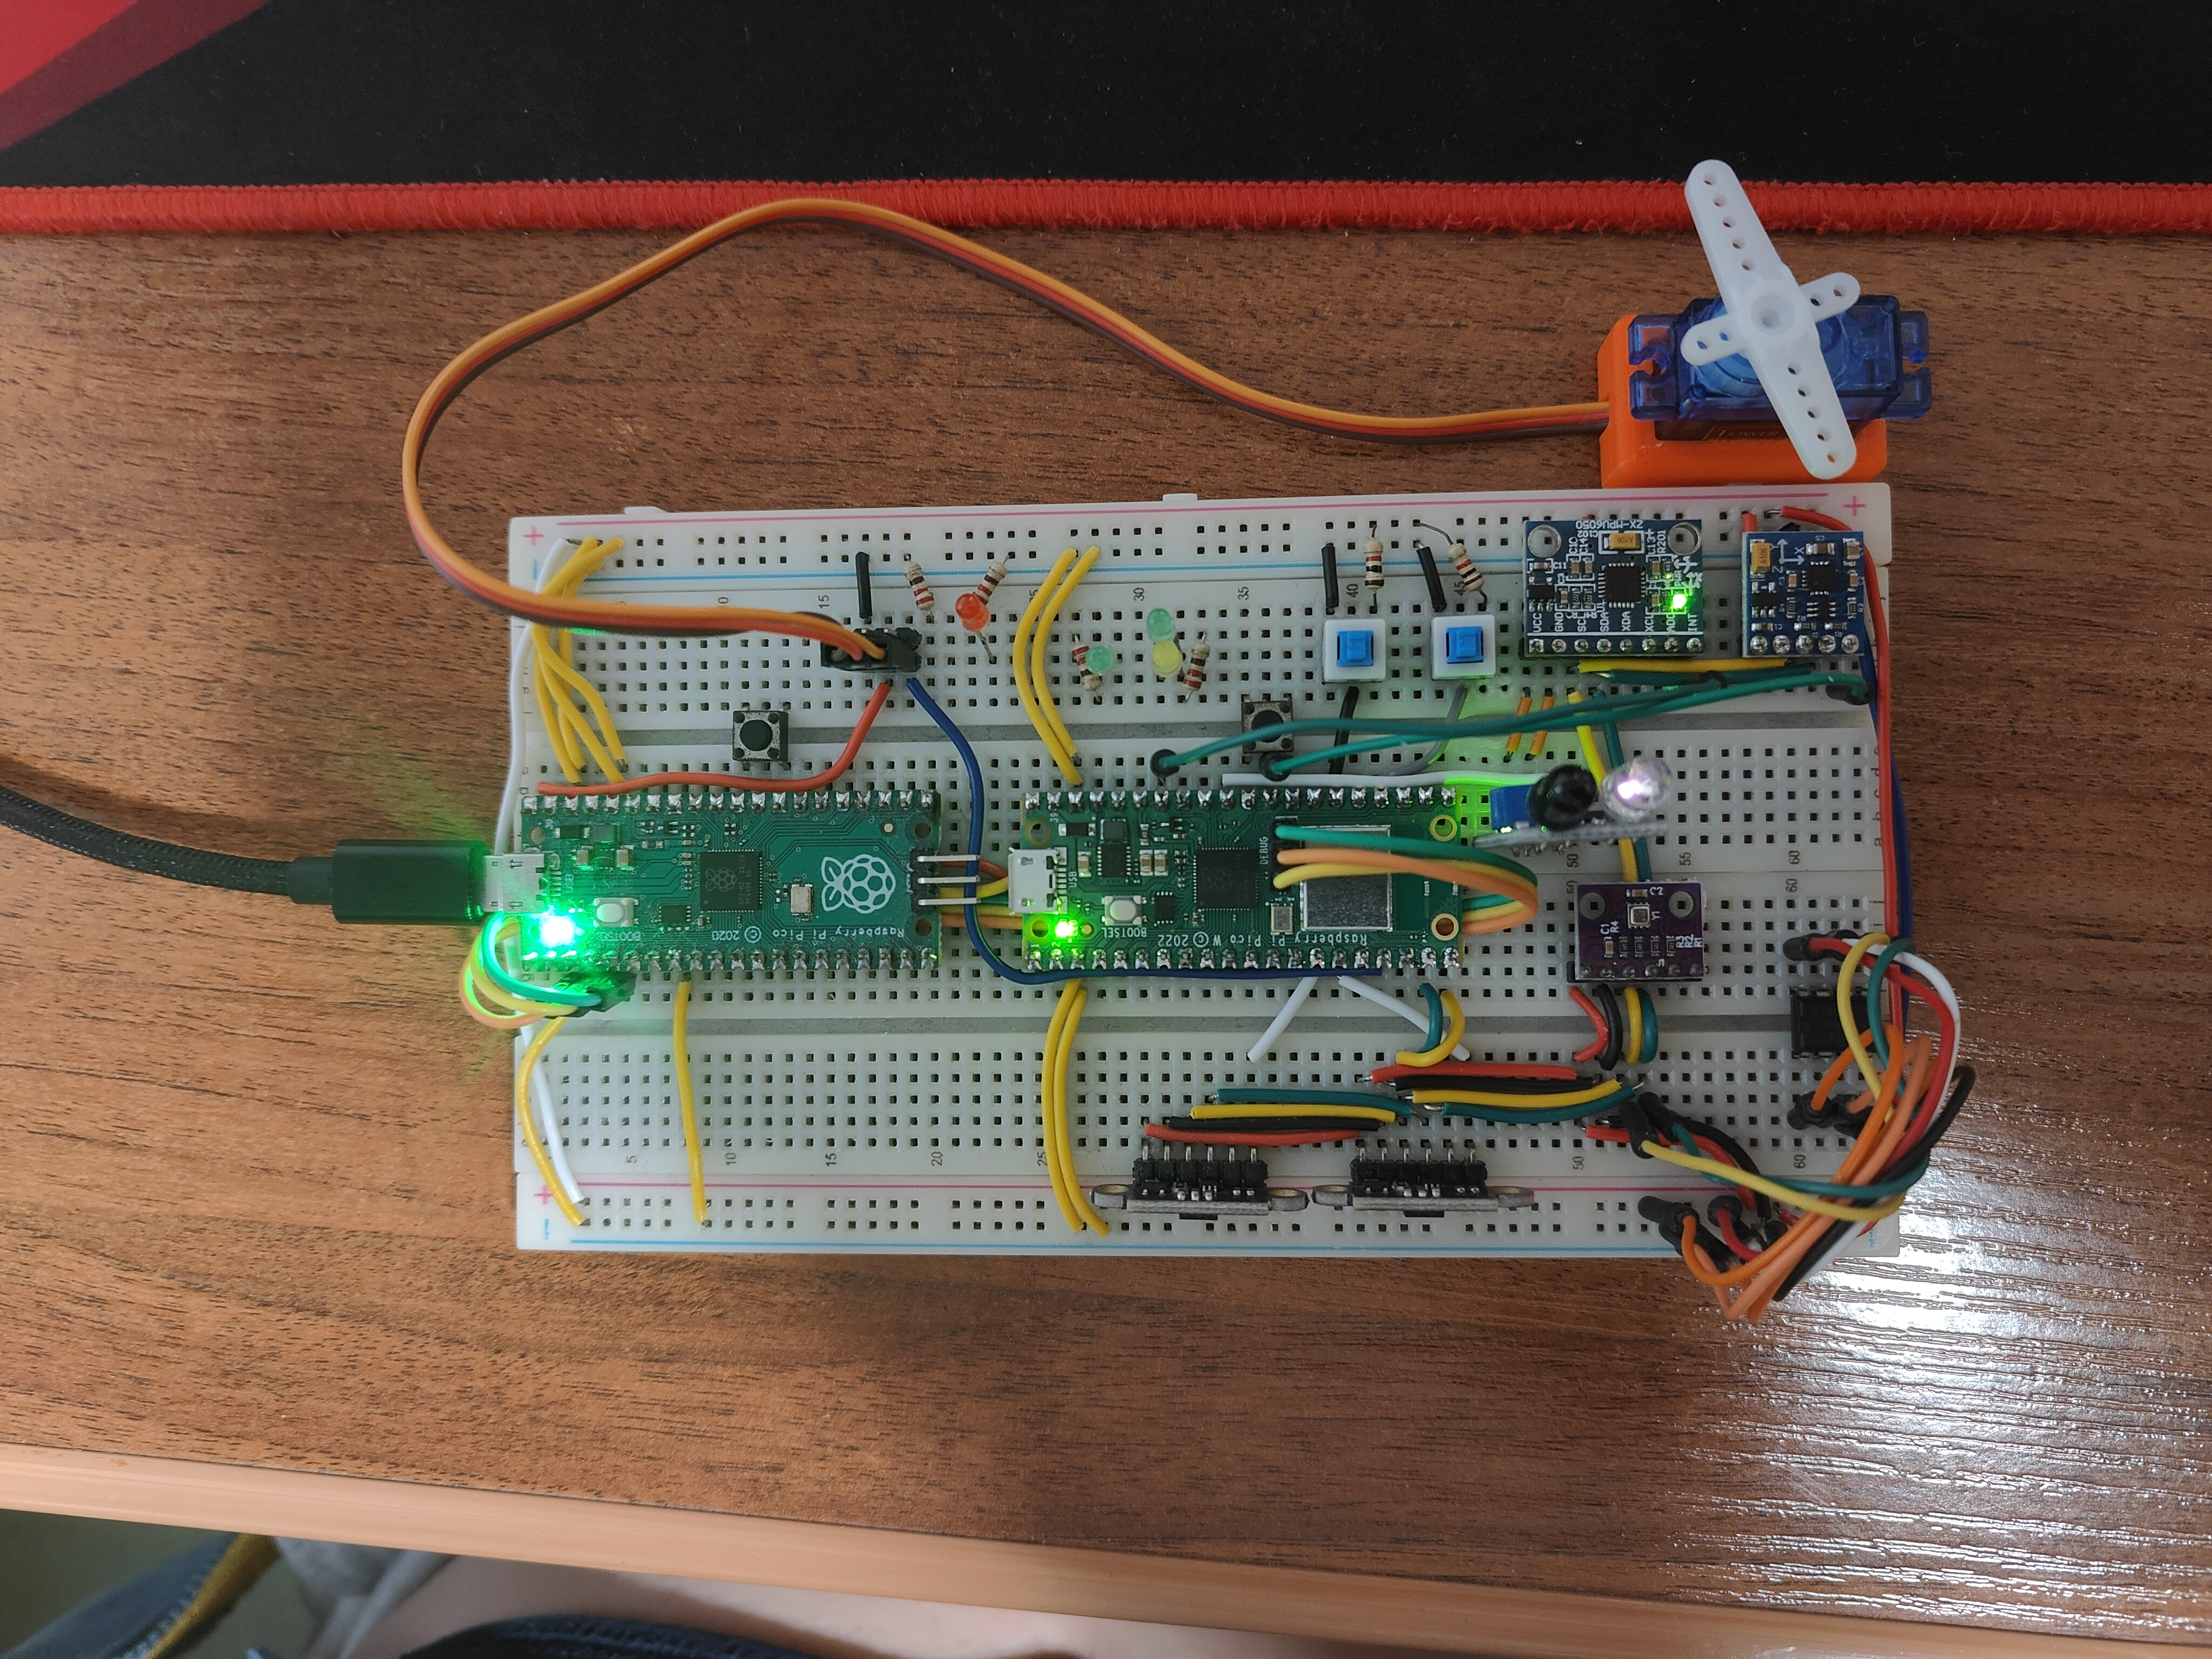
\includegraphics[width = 0.7\textwidth, trim = {500px, 500px, 350px, 350px}, clip]{Breadboard.jpg}
            \caption{Model prototypowy na płytce stykowej}
            \label{fig:breadboard}
        \end{figure}

        Zbudowany model z płytki stykowej, został skompresowany aby zmieścił się na pojedynczej płytce o rozmiarach 400-stu pól.
        Tak ściśnięty układ można było założyć na ramę pojazdu.
        W tym celu została zaprojektowana i wydrukowana mała podpora, która pozwoliła na sztywne zamocowanie układu.

        \begin{figure}[!ht]
            \centering
            \includegraphics[width = 0.7\textwidth, trim = {800px, 400px, 1200px, 200px}, clip]{Breadboard_car.jpg}
            \caption{Model pojazdu z zainstalowaną płytą prototypową}
            \label{fig:breadboard_car}
        \end{figure}

        Po zamocowaniu płytki stykowej do prototypowej ramy, pojazd został poddany testom jednostkowym.
        Testy te polegały na sprawdzeniu działania wszystkich komponentów.
        Następnie, sprawdzono działanie podstawowych funkcji, typu jazda czy skręcanie.

        Podczas testowanie elementów pojedynczo, wszystko działało poprawnie.
        W czasie dłuższych testów, okazało się, że układ akcelerometru, potrafi zawiesić się w losowym momencie.
        Rozwiązaniem tego problemu, w tej wersji projektu, okazało się niemożliwe, ze względu na działanie płytki stykowej.
        Podczas jazdy, cały pojazd drżał, co powodowało, że niektóre piny nie stykały i układ akcelerometru, po spadku zasilania, blokował magistralę $I^2C$.

        Problematyczna okazała się linia $SDA$, protokołu $I^2C$.
        Rozwiązanie tego problemu było trudnym zadaniem.
        Szczególnie że bardzo ciężko było wykryć pierwotną przyczynę zawieszania się układu.
        Pierwszym rozwiązaniem problemu, było zastosowanie się do instrukcji z noty aplikacyjnej od Analog Devices o resetowaniu linii $I^2C$ \cite{application_note_I2C_AD}.
        Podobne rozwiązanie można znaleźć w dokumentacji do magistrali $I^2C$ \cite{I2C_manual_NXP} wydanej przez NXP.
        Niestety, zastosowane rozwiązanie nie przyniosło oczekiwanych rezultatów.

        Drugim rozwiązaniem sugerowanym przez oba dokumenty, w sytuacji kiedy nie udało się odblokować magistrali jest zresetowanie niedziałających (w domyśle wszystkich) układów.
        To rozwiązanie, mimo swojej skuteczności nie zostało wykorzystane.
        Autor skupił się na znalezieniu pierwotnej przyczyny problemu.

        Dodatkową zaletą wykonanie w pierwszej wersji projektu na płytce stykowej oraz losowego zawieszania się programu, było udoskonalenie funkcji odpowiedzialnych za kontrolę protokołu $I^2C$.
        W pierwszej wersji programu, komunikacja $I^2C$, blokowała pracę procesora.
        Rozwiązanie to sprawdzało się tak długo jak wszystko działało poprawnie.
        Jednak luźne połączenia ukazały, że to rozwiązanie jest niepraktyczne.
        W drugiej wersji programu, instrukcje odpowiedzialne za komunikację $I^2C$ zostały ograniczone \textit{timeoutem}.

        Ostateczną wersją prototypu jest płytka prototypowa, zlutowana na stałe.
        Zlutowanie układu na płytce, pozwoliło pozbyć się niektórych problemów, przykładowo blokowania się magistrali $I^2C$.
        Jednak złożenie zlutowanej wersji objawiło inne problemy, które ukrywała płytka stykowa.
        \begin{figure}[!ht]
            \centering
            \includegraphics[width = 0.7\textwidth, trim = {500px, 300px, 300px, 200px}, clip]{Protoboard_car.jpg}
            \caption{Model pojazdu z zainstalowaną płytą prototypową}
            \label{fig:protoboard_car}
        \end{figure}

        Największym problemem, który pojawił się po zlutowaniu prototypu, było losowe resetowanie się RB Pi Pico (Raspberry Pi Pico).
        Znalezienie przyczyny tego problemu okazało się trudne.
        Problem występował czasami zarówno po podłączeniu zewnętrznego zasilacza jak i pracy na akumulatorach.
        Po testach okazało, się że sytuacja ta występuje tylko wtedy, gdy pracują silniki oraz podłączone są enkodery.
        Po odłączeniu wyjść sygnałowych enkoderów, kłopot z resetowaniem się układu zniknął.
        W celu upewnienia, się że przyczyną są uszkodzone enkodery, w szereg z wyjściem sygnałowym został podłączony rezystor o rezystancji $R =1k\Omega$.
        Po podłączeniu rezystora, problem z resetowaniem się układu zniknął na kilka dni.
        Po czym powrócił. Szukając problemów w okolicy silników, zostało zmienione zasilanie silników na niezależne od reszty układu.
        Uruchomienie silników, z zasilaniem niezależnym natychmiast zresetowało procesor.
        Kolejną próbą była zmiana mostka H na inny. Wymiana tego układu również nie pomogła.
        W między czasie podczas składania prototypu, uszkodzeniu uległ jeden z układów ToF.
        Po wymianie uszkodzonego układu, problem z resetowaniem się RB Pi Pico nie zniknął.
        Ostatnim pomysłem co mogło zostać uszkodzone, była sama malinka, jednak jej wymiana również nie pomogła.
        Ostatecznie, rozwiązaniem okazało się dołożenie dużej roznoszonej pojemności (około $500\mu F$) na całej płytce.

        Kolejnym problemem, na który natrafił autor, były oscylacje na liniach przerwań od czujników obiektów zamontowanych na tyle pojazdu.
        Oscylacje te, nie pozwalały na poruszanie się do tyłu, ponieważ czujniki w losowych momentach zgłaszały obiekt i zatrzymywały silniki.
        Rozwiązaniem tego problemu było zastosowanie filtru RC, który niweluje drgania.



    \subsection{Automatyzacja praca}
        Automatyzacja pracy jest niezwykle ważnym zadaniem w momencie, testowania podstawowych funkcji.
        Oczywiście, każdą funkcję można wywołać ręcznie, jednak podczas testów, kiedy wielokrotnie wykonywane są podobne funkcje, automatyzacja staje się obowiązkowa.

        Aby wykonać to zadanie, w języku Python został napisany skrypt, który pozwala na dwustronną komunikację za pomocą protokołu $UDP$.
        Dodatkowo, program pozwala na interpretację plików, napisanych specjalnie dla tego układu.
        Poniżej przedstawiono listing \eqref{list:self_test.s} programu do testowania podstawowych działań pojazdu.

        \lstinputlisting[style=asm, caption={Test pojazdu}, label = list:self_test.s]{Listing/self_test.s}

        \subsubsection{Interpreter własnego języka}
            Przedstawiony w listingu \ref{list:self_test.s} program jest interpretowanym przez skrypt napisany w pythonie.
            Jego zadaniem jest stokenizowanie instrukcji, wyznaczanie adresów skoków oraz stworzenie słownika z zmiennymi.
            Następnie, program przechodzi do wykonywania instrukcji zapisanych w pliku.
            Powyższy język posiada tylko kilka prostych słów kluczowych przedstawionych w tabeli \ref{table:keywords}.
            Pozostałe instrukcje po sformatowaniu wysyłane są do malinki.

            \begin{table}[!ht]
                \centering
                \caption{Lista słów kluczowych do mini języka}
                \begin{tabularx}{0.8\textwidth}{|c|c|C|}\hline
                    Nr. & Instrukcja & Opis \\\hline
                     1. & jump $etykieta$ & Skok do $etykiety$ \\\hline
                     2. & end & Koniec programu lub funkcji \\\hline
                     3. & print $zmienna/napis$ & Wypisanie wartości zmiennej lub napisu\\\hline
       \centerY{2}{ 5.} & \centerY{2}{if $warunek$} & Instrukcja warunkowa, w przypadku nie spełnienia pomija następną instrukcję\\\hline
       \centerY{2}{ 7.} & \centerY{2}{$etykieta$\textbf{:}} & Etykieta funkcji, koniecznie zakończona znakiem ,,:''\\\hline
       \centerY{4}{ 9.} & \centerY{4}{$\$zmienna$} & Odwołanie do zmiennej w przypadku instrukcji wysłanych. Podczas formatowania instrukcje, $\$zmienna$ zostaje podmieniona na wartość\\\hline
       \centerY{2}{10.} & \centerY{2}{$zmienna$ = \textit{wartość}} & Przypisanie wartości do zmiennej. Pozwala na wykonywanie operacji matematycznych\\\hline
                \end{tabularx}
                \label{table:keywords}
            \end{table}

            Wszystkie pozostałe instrukcje, które nie są zdefiniowane w tabeli, wysyłane są bezpośrednio do mikrokontroler.
            Natomiast w przypadku, kiedy instrukcja zostaje odnaleziona, ale zawiera błąd składniowy, program wyświetla błąd i przerwa działanie.
            Przykład takiej sytuacji przedstawiono na rysunku \ref{fig:interpreter}.

            \begin{figure}[!ht]
                \centering
                \includegraphics[width = 0.7\textwidth]{Terminal_program_testowy.png}
                \caption{Program zawierający celowe błędy}
                \label{fig:interpreter}
            \end{figure}

            W przypadku, kiedy program pracuje poprawnie, instrukcje wypisywane są równolegle z wiadomościami odebranymi od samochodu.
            Rozkazy wysyłane do mikrokontrolera, są poprzedzone łańcuchem znaków ,,$>>>$''.
            Natomiast instrukcja wynik instrukcji $print$ jest identyczny z tym, co zwraca mikrokontroler.
            Podczas testowania programy, program zdążył wysłać kilka instrukcji do raspberry dlatego po zgłoszeniu błedy widnieją widnieje kilka odebranych instrukcji.
    \section{Problemy konstrukcyjne}
\label{sec:problemy_konstrukcyjne}
    W poniższym rozdziale zostaną przedstawione problemy konstrukcyjne,
    które pojawiły się podczas realizacji projektu.

    \subsection{Jazda prosto}
    \label{section:jazda_prosto}
        Najprostszą czynnością każdego pojazdu jest jazda prosto.
        Operacja ta może wydawać się łatwa jednak wcale taka nie jest.
        Przykładowo kiedy usiądziemy za kierownicą, prawdziwego samochodu kontroluje podświadomie wiele parametrów takich jak:
        \begin{itemize}
            \item nachylenie terenu,
            \item aktualną pozycję kół,
            \item linie poziome na drodze czy pobocze drogi.
        \end{itemize}
        Jako ludzie wiele tych parametrów kontroluje ,,na wyczucie'' jednak pojazdy autonomiczne, są poniekąd robotami, które nie mogą polegać na ,,uczuciu'', że jadą prosto.
        Dlatego koniecznym jest zastosowanie odpowiednich czujników, które pozwolą na dokładną kontrolę jazdy.
        W poniższym rozdziale pokrótce zostaną opisane rozwiązanie dzięki którym samochód jest w stanie jeździć w sposób powtarzalny.

        \subsubsection{Różnica prędkości silników}
            Zastosowanie dwóch silników ma swoje wady i zalety.
            Niewątpliwą zaletą jest podwojenie mocy pojazdu.
            Jednak olbrzymią wadą okazało się sterowanie i nierównomierność pracy silników.
            Na wykresie \ref{plot:distance_err_in_time_const_speed} poniżej przedstawiono różnicę drogi pokonanej przez każdy silnik dla jednakowego sygnału sterującego.

            \begin{figure}[!ht]
                \centering
                \begin{tikzpicture}
                    \begin{axis}[
                        width = 0.7\textwidth,
                        grid = both,
                        grid style = dashed,
                        % axis lines = middle,
                        xlabel = czas ${[s]}$,
                        ylabel = różnica odległości ${[mm]}$,
                        xmin = 0,
                        xmax = 20,
                    ]
                        \addplot[blue] table[x = Time, y = Diff, col sep = comma]{Measure/distance_no_PID_speed_50.csv};
                        \legend{Błąd odległości}
                    \end{axis}
                \end{tikzpicture}
                \caption{Wykres różnicy przebytej drogi między prawym a lewym silnikiem bez regulacji}
                \label{plot:distance_err_in_time_const_speed}
            \end{figure}

            Aby rozwiązać powyższy problem należy zastosować regulator PID pozwalający w trakcie pracy, korygować prędkość silników.
            Natomiast podczas startu silników została zastosowana sztywna korekta prędkości w celu zminimalizowania błędu.
            \begin{figure}[!ht]
                \centering
                \begin{tikzpicture}
                    \begin{axis}[
                        width = 0.7\textwidth,
                        grid = both,
                        grid style = dashed,
                        xlabel = czas ${[s]}$,
                        ylabel = różnica odległości ${[mm]}$,
                        xmin = 0,
                        xmax = 60,
                    ]
                        \addplot[blue] table[x = Time, y = Distance_err, col sep = comma]{Measure/PID_speed_10.csv};
                        \legend{Błąd odległości}
                    \end{axis}
                \end{tikzpicture}
                \caption{Wykres różnicy przebytej drogi między prawym a lewym silnikiem z włączonym regulatorem PID. Prędkość pojazdu: $(35.10 \pm 0.10)\frac{mm}{s}$.}
                \label{plot:PID_distance_err_in_time}
            \end{figure}

            Jak widać na wykresie \ref{plot:PID_distance_err_in_time} w początkowej fazie, silniki nadal nie pracują równomiernie, w dłuższej perspektywie praca silników osypuje w okół stałej wartości $(0 \pm 3)mm$.

    \subsubsection{Nieidealność podwozia}
        Kolejnym napotkanym problemem, okazuje się nieidealność podwozia.
        Szczególnie elementu przedstawionego na rysunku \ref{fig:frontAxis_model} oraz nierównomierne rozłożenie masy względem środka.
        Wszystkie wyżej wymienione niedokładności powodowały, że pojazd cały czas skręcał w jedną stronę.
        Rozwiązaniem tego problemu jest zastosowanie pętli sprzężenia zwrotnego, opartej na czujniku $MPU6050$, który został użyty jak żyroskop, pozwalający na pomiar biedzącego kąta.
        Dzięki czemu można korygować kierunek skręcania pojazdu.

        Jednak jego wykorzystanie nie było bezproblemowe i wymagało dodatkowych poprawek.
        Na wykresie \ref{plot:gyro_magneto_measure} przedstawiono pomiar kąta dla obrotu pojazdu ze stałą prędkością w jednym kierunku po kalibracji czujnika.
        Poniższy pomiar został wykonany w celu ustalenia liniowości pracy żyroskopu opartego na akcelerometrze.
        Układem referencyjnym był uprzednio skalibrowany magnetometr (układ $QMC5883L$).
%
        \begin{figure}[!ht]
            \centering
                \begin{tikzpicture}
                    \begin{axis}[
                        width = 0.65\textwidth,
                        grid = both,
                        grid style = dashed,
                        xlabel = czas ${[s]}$,
                        ylabel = kąt zmierzony podczas obrotu ${[^\circ]}$,
                        ymin = -5,
                        ymax = 365,
                        xmin = 0,
                        xmax = 2.9,
                        ytick = {0, 30, ..., 360},
                        legend style={at={(0.2, 0.92)}, anchor=north},
                    ]
                        \addplot[orange] table[x = Time, y = Compass_azimuth, col sep = comma]{Measure/angles.csv};
                        \addplot[blue] table[x = Time, y = Gyro_z, col sep = comma]{Measure/angles.csv};
                        \legend{magnetometr,żyroskop}
                    \end{axis}
                \end{tikzpicture}
                \caption{Wykres pomiary azymutu za pomocą magnetometru oraz zmiany kąta wykazanego przez żyroskop}
                \label{plot:gyro_magneto_measure}
        \end{figure}
        Podczas pomiaru, na oba układy został nałożony filtr dolnoprzepustowy, eliminujący szumy.

        Wykres \ref{plot:delta_angle_with_gyro} przedstawia narastanie katą, mierzonego przez żyroskop.
        Widać bardzo dużą liniowość pracy żyroskopu, co pozwala zaufać temu czujnikowi na tyle, aby na jego podstawie określać czy pojazd jedzie prosto.

        % \begin{wrapfig}[!ht]
        \begin{figure}[!ht]
            \centering
                \begin{tikzpicture}
                    \begin{axis}[
                        width = 0.7\textwidth,
                        grid = both,
                        grid style = dashed,
                        xlabel = czas ${[s]}$,
                        ylabel = kąt zmierzony podczas obrotu ${[^\circ]}$,
                        xmin = 0,
                        xmax = 2.9,
                    ]
                        \addplot[blue] table[x = Time, y = Delta_angle, col sep = comma]{Measure/angles.csv};
                    \end{axis}
                \end{tikzpicture}
                \caption{Wykres narastania kąta, zmierzonego przez żyroskop}
                \label{plot:delta_angle_with_gyro}
        \end{figure}
        % \end{wrapfig}


% \newpage
    Oba wyżej opisane rozwiązania pozwalają na w miarę stałą jazdę prostą ($\pm 2^\circ$).
    A w sytuacjach, kiedy pojazd zaczyna znacząco skręcać na przykład po impakcie z boku, sprzężenie zwrotne z żyroskopu pozwala wykryć znaczącą zmianę kąta ruchu.
    Kolejny regulator PID odczytuje wartość kąta i koryguje kąt serwomechanizmu tak aby pojazd wrócił na prostą.

    \subsection{Skręcanie}
        Rozwiązanie problemów z jazdą prosto to tylko połowa sukcesu.
        Kolejne mankamenty wyszły podczas próby skręcania.
        Nie tylko w pierwotnej wersji nie było stałe - ustawienie stałego kąta kół oraz przejechanie tej samej drogi nie zawsze dawało ten sam rezultat.
        To pojazd cały czas miał tendencję do preferowania skrętu w jedną stronę.

        \subsubsection{Dyferencjał}
        \label{subsubsec:dyferencjal}
        Najprostszym do zauważenia problemem był brak dyferencjału.
        Tylna oś pojazdu posiada dwa silniki jednak w poprzednich testach, zostały one ,,software'owo połączona sztywną belką".
        Powodowało to poślizg pojazdu podczas skręcania a w konsekwencji uniemożliwiało powtarzalność manewru.

        Rozwiązaniem tego problemu jest zmiana prędkości pracy silników w zależności od promienia skrętu.
        Poniżej przedstawiono schemat algorytmu, na którego podstawie wyznaczono procentową wartość dyferencjału.
        Rysunek \ref{draw:turning_car} przedstawia schematyczną sytuację skręcania.
        \begin{figure}[!ht]
    \centering
    \begin{tikzpicture}
        \draw
            (0, 0) node[draw, rectangle, rounded corners, fill = black, minimum width = 2cm, minimum height = 0.8cm, rotate = 30](frontL){}
            (0, -3) node[draw, rectangle, rounded corners, fill = black, minimum width = 2cm, minimum height = 0.8cm, rotate = 30](frontR){} 
            
            (6, 0) node[draw, rectangle, rounded corners, fill = black, minimum width = 2cm, minimum height = 0.8cm](backL){}
            (6, -3) node[draw, rectangle, rounded corners, fill = black, minimum width = 2cm, minimum height = 0.8cm](backR){}

            (3, 0) node[above]{Prawa strona}
            (3,-3) node[below]{Lewa strona}
        ;

        \draw[Stealth-Stealth]
            (frontL) ++ (0, 1) --node[above]{$l$}++ (6, 0)
        ;
        \draw[dashed, gray]
            (frontL) --++(0, 1)
            (backL) --++(0, 1)
        ;

        \draw[color = red]
            (backL) -- ++ (0, -10) -- ++ (0, -1) coordinate(meet) --++ (0, -1)
            (frontL) -- (meet)
            (frontR) -- (meet)
        ;
        \draw
            (meet) ++ (0, 3) arc(90:127:3) node[above]{$\alpha$}
            (meet) ++ (0, 2) arc(90:147:1) node[above]{$\beta$}
        ;

        \draw[dotted]
            (backL) to[short, l=$\Delta r$] (backR)
            (backR) ++ (0, -2.5) node[right]{$r$}
        ;

        \draw[dashed]
            (frontL) ++ (0, 1) -- (0, -5)
            (0, -4) arc(90:180:-1)
            (0.5, -4.5) node[]{$\gamma$}
            (1.2, -4.25) node[rotate = -50]{$90 - \gamma$}
        ;
    \end{tikzpicture}
    \caption{Rysunek poglądowy do skręcenia}
    \label{fig:turning_car}
\end{figure}

        Jak widać skręt pojazdu można opisać jako ruch dwóch kół po okręgach o wspólnym środku, w których poszczególne prędkości liniowe nie są sobie równe.
        Jednak występuje zależność:
        \begin{gather}
            \omega_{\text{wewnęrznego koła}} = \omega_{\text{zewnętrznego koła}}\\
            \frac{v_{\text{wewnęrznego koła}}}{r} = \frac{v_{\text{zewnętrznego koła}}}{r + \Delta r}\\
            \frac{v_\text{wewnęrznego koła}}{v_{\text{zewnętrznego koła}}} = \frac{r}{r + \Delta r}
        \end{gather}

        Aby policzyć zależność między prędkościami silników, należy wyznaczyć promień skrętu.
        Do tego celu, można wykorzystać znane wartości i równanie \ref{eq:turning_radius}.
        Znanymi wartościami są:
        \begin{gather}
            \tan \left(90 - \gamma\right) = \frac{l}{r}\\
            r(\gamma) = \frac{l}{\tan(90-\gamma)}
            \label{eq:turning_radius}
        \end{gather}

        Gdzie:
        \begin{itemize}
            \item $l = 155$ -- długość między osiami samochodu:,
            \item $\Delta r = 125$ -- odległość między kołami w jednej osi,
            \item $\gamma \in <60^\circ \div 120^\circ>$ -- kąt skrętu kół, ustawiany przez algorytm nawigacji lub użytkownika.
        \end{itemize}

        A zatem procentowy stosunek prędkości w funkcji kąta można wyrazić jako:
        \begin{gather}
            \frac{v_{\text{prawe koła}}}{v_{\text{lewe koła}}} = 1 + \frac{\Delta r}{r} = 1 + \Delta r \cdot \frac{\tan(90 - \gamma)}{l}
        \end{gather}


        \subsection{Nierównomierność skrętu}
        \label{subsec:nierownomiernosc_skretu}
            W trakcie testów, okazało się że pojazd nie skręca równomiernie w obie strony.
%
            Podczas manewrów w prawo, na łuku o długości $s = 500mm$, pojazd zakreślał kąt około $70^\circ$.
            Natomiast na tym samym odcinku ale w lewo zakreślany kąt to około $50^\circ$.

            Wymusiło ustawienie wartości offsetu, przesuwającej wartość kąta skrętu.
            Jego wartość została wyznaczona eksperymentalnie i wynosiła około $-6^\circ$.
            Dla podanej wartości kąt zakreślany podczas skrecania w obu kierunkach wynosił około $60^\circ$.



    Dzięki wszystkim wyżej wymiennym zabiegom udało się uzyskać powtarzalne wyniki zarówno podczas jazdy prosto, cofania się oraz skręcania.
    Powyższe działania są niezbędne, jeśli budowany robot ma być sterowany autonomicznie.


    \section{Sterowanie pojazdem}
    Sterowanie pojazdem powinno odbywać się w sposób płynny i precyzyjny.
    W poniższym rozdziale zostaną omówione algorytmy odpowiedzialne za najbardziej podstawowe funkcje poruszania się takie jak: jazda prosto, skręt oraz cofanie.

    \subsection{Jazda przez pewien odcinek}
    \label{subsec:jazda_przez_odcinek}
        W rozdziale \ref{section:jazda_prosto} zostały opisane problemy jakie wystąpiły podczas budowy pojazdu. %oraz problemy jakie musiały zostać rozwiązane aby samochód był w stanie jechać prosto.
        Dzięki ich rozwiązaniu możliwa była jazda prosto.
        Jednak dla precyzyjnego sterowania informacja o tym, że pojazd porusza się po linii prostej jest niewystarczająca.
        Obowiązkowym staje się poznanie odległości jaka została pokonana.

        Dystans jaki pokonuje pojazd od momentu startu, możemy dość dokładnie obliczyć korzystając ze wzoru \eqref{eq:pulseToDistance}.
        \begin{gather}
            s = \frac{\text{pulse} \cdot 2\pi R}{N}
            \label{eq:pulseToDistance}
        \end{gather}
        gdzie:
        \begin{itemize}
            \item $s$ -- odległość jaką pokonał pojazd,
            \item $\text{pulse}$ -- liczba impulsów z enkodera,
            \item $R$ -- promień koła,
            \item $N$ -- liczba impulsów na obrót koła.
        \end{itemize}

        Wzór ten można także przekształcić w drugą stronę, aby obliczyć ile impulsów enkodera musi zostać zliczonych przez procesor aby pojazd pokonał zadaną odległość.
        \begin{gather}
            \text{pulse} = \frac{s \cdot N}{2\pi R}
            \label{eq:distanceToPulse}
        \end{gather}

        Dla zbudowanego modelu promień koła wynosi $R = 50cm$ a liczba impulsów zgodnie z dokumentacją wynosi $N = 1920$.
        A więc dokładność pomiaru odległości wynosi około:
        \begin{gather}
            \Delta s \approx \pm2.0mm
        \end{gather}

        Dzięki zastosowaniu równania \eqref{eq:distanceToPulse}, możliwe jest wysłanie informacji do pojazdu aby po określonej ilości impulsów z enkoderów, zatrzymał się.


    \subsection{Wyznaczanie zakrętów}
        Wyznaczenie idealnie prostej trasy dla pojazdów nie zawsze jest możliwe.
        W trakcie jazdy, samochód będzie skręcał wielotonie, w każdym możliwym kierunku.
        Przedstawiony model posiada dwie osiowe, przez co nie jest w stanie wykonać tego manewru w miejscu.
        Natomiast może swobodnie poruszać się po okręgu o minimalnym promieniu.
        W tym rozdziale zostanie opisany sposób wyznaczania tego promienia w zależności od kąta skrętu kół.

        \subsubsection{Minimalny promień skrętu}
        \label{subsubsec:minamalny_promien}
            Wykorzystując rysunek \ref{draw:turning_car} oraz zależność \eqref{eq:turning_radius}, można obliczyć minimalny promień skrętu.
            Po podstawieniu wartości do wzoru, otrzymujemy:
            \begin{gather}
                r(\gamma = 90 \pm 30^\circ) = \left|\frac{155}{\tan(\pm 30^\circ)}\right| \approx 270mm
                \label{eq:theoretical_radius}
            \end{gather}

            Otrzymaną wartość należy jednak skonfrontować z rzeczywistością.
            W tym celu przedstawiono inny sposób wyznaczenia promienia skrętu.
            Równanie \eqref{eq:turning_arc} pozwala na obliczenie tego parametru na podstawie zakreślonego kąta i długości łuku.
            \begin{gather}
                s = 2\pi (r(\gamma) + \Delta r) \cdot \frac{\alpha}{360}
                \label{eq:turning_arc}
                % \\
                % \alpha = \frac{2\pi (r(\gamma + \Delta r))}{s \cdot 360}
            \end{gather}
            gdzie:
            \begin{itemize}
                \item $s$ -- długość łuku,
                \item $r(\gamma)$ -- promień skrętu dla danego skrętu kół,
                \item $\Delta r$ -- odległość między kołami,
                \item $\alpha$ -- oczekiwany kąt skrętu.
            \end{itemize}

            Przekształcając powyższe równanie otrzymujemy zależność:
            \begin{gather}
                r(\gamma) = \frac{s}{2\pi \cdot \frac{\alpha}{360}} - \Delta r
                \label{eq:turning_radius_with_arc}
            \end{gather}

            Odległość pokonana przez samochód jest dość precyzyjne mierzona przez enkodery.
            A zakreślony kąt został zmierzony przez wcześniej skalibrowany akcelerometr.
            Dzięki czemu można uznać, że zadana długość łuku i zakreślony kat są precyzyjne.

            Przykładowo dla ustawionego maksymalnego kąta skrętu kół $\gamma = 90 + 30^\circ$ oraz długości łuku $s = 500mm$, wartość zakreślonego kąta wynosiła około $\alpha = 60.0^\circ$.
            Podstawiając podane wyniki do równania \eqref{eq:turning_radius_with_arc}, otrzymujemy:
            \begin{gather}
                r = \frac{500mm}{2\pi \cdot \frac{60}{360}} - 125mm \approx (350)mm
            \end{gather}


            Teoretyczny minimalny promień skrętu wychodzący z obliczeń (równanie \eqref{eq:theoretical_radius}), jest znacząco mniejszy od zmierzonego minimalnego promienia skrętu.
            Wynika to z nie idealności konstrukcji oraz zastosowania ,,względnie słabej jakości'' serwomechanizmu.
            Co ogranicza maksymalny zakres skrętu do $\pm 24^\circ$.
            \begin{gather}
                r(\gamma = 90 + 24^\circ) = \left|\frac{155}{\tan(+ 24^\circ)}\right| \approx 350mm
            \end{gather}

            Jednak po uwzględnieniu zależności z rozdziału \ref{subsec:nierownomiernosc_skretu}, okazuje się że różnica między teoretycznym a obliczonym kątem skrętu kół wynosi dokładnie wartość offsetu ($-6^\circ$).
            Dlatego też ograniczenie skrętu kół do $\pm 24^\circ$ nie jest potrzebne. 
            I w późniejszych obliczeniach kąt skrętu kół brany pod uwagę będzie w zakresie $\pm 30^\circ$.



    \section{Mapa i orientacja przestrzenna}
    W celach testowych została napisana dedykowana aplikacja graficzna do sterowani pojazdem oraz reprezentująca mapę użytkownikowi.
    Na zdjęciu \ref{fig:app} przedstawiono interfejs aplikacji.
    \begin{figure}[!ht]
        \centering
        \includegraphics[width = 0.7\textwidth]{PathFinding/App.png}
        \caption{Interfejs aplikacji}
        \label{fig:app}
    \end{figure}
    Interfejs aplikacji składa się z trzech części:
    \begin{enumerate}
        \item Mapa -- reprezentująca aktualnie zbadanego obszar oraz aktualną pozycję pojazdu.
        \item Informacje -- w prawym górnym rogu, wyświetlane są dodatkowe informacje, takie jak aktualna pozycja pojazdu, czy myszy.
        \item Ślizgacze -- w prawym dolnym rogu, znajdują się dwa ślizgacze, górny pozwala precyzyjnie ustawić kąt skrętu kół a dolny pozwala na ustawienie prędkości pojazdu.
    \end{enumerate}

    \subsection{Budowa mapy}
        W założeniu aplikacja ma pozwalać jedynie na wyświetlanie, mapy zbudowanej przez samochód.
        Natomiast wszystkie obliczenia powinny zostać wykonane przez kontroler zarządzający pojazdem.
        Jednak ze względu na duże skomplikowanie opisywanych problemów, w celach testowych, to aplikacja posiada zaimplementowany algorytm do wyszukiwania ścieżek.
        Następnie wyznaczona ścieżka zamieniana jest na proste instrukcje w stylu ,,uruchom oba silniki na 500mm'' czy ,,skręć kołami o $30^\circ$ w lewo''.




    \subsection{Wyznaczanie ścieżek}
        Kliknięcie na mapę, pozwala na wybranie punktu docelowego, do które zostanie wyznaczona ścieżka, po której pojazd będzie się poruszał.
        Dzięki zastosowaniu algorytmu Dijkstry opisanego w rozdziale \ref{subsec:algorytm_odnajdowania_ścieżek}, możliwe jest wyznaczcie optymalnej ścieżki.
        Następnie wyznaczona ścieżka zamieniana jest na instrukcje ruchu.

        \subsubsection{Algorytm odnajdowania ścieżek}
        \label{subsec:algorytm_odnajdowania_ścieżek}
            Wyznaczanie optymalnej ścieżki, od wielu lat jest bardzo popularnym problemem w informatyce i robotyce.
            Istnieje wiele artykułów, skupiających się na tej tematyce, a także wiele gotowych rozwiązań.
            Najpopularniejszymi algorytmami są:
            \begin{itemize}
                \item algorytm A* (A star),
                \item algorytm Dijkstra,
                \item algorytm Bellmana-Forda.
            \end{itemize}

            Poniżej przedstawione zostaną wyniki pracy \citetitle{AnalizaAlgorytmówŚcieżek} \cite{AnalizaAlgorytmówŚcieżek}
            autorstwa: Beata \citeauthor{AnalizaAlgorytmówŚcieżek}.
            \begin{figure}[!ht]
                \centering
                \figurePlotName
                \includegraphics[width=0.7\textwidth]{PathFinding/Wykres_sredni_czas_algorytmu_pathfinding.png}
                \caption{Porównanie średniego czasu wykonania algorytmów}
                Źródło:\cite{AnalizaAlgorytmówŚcieżek} \citetitle{AnalizaAlgorytmówŚcieżek}
                \label{fig:PathFindingTime}
            \end{figure}
            \begin{figure}[!ht]
                \centering
                \figurePlotName
                \includegraphics[width=0.7\textwidth]{PathFinding/Wykres_sredni_koszt_algorytmu_pathfinding.png}
                \caption{Porównanie średniego kosztu znalezionych ścieżek}
                Źródło:\cite{AnalizaAlgorytmówŚcieżek} \citetitle{AnalizaAlgorytmówŚcieżek}
                \label{fig:PathFindingCost}
            \end{figure}

            Z powyższej pracy wynika, że najlepszym rozwiązaniem jest algorytm Dijkstry.
            Dodatkowym czynnikiem, potwierdzającą powyższe stwierdzenie jest samo skomplikowanie algorytmu.
            Algorytm Dijkstry jest stosunkowo prosty w implementacji, a także posiada niski koszt obliczeniowy.
            Dzięki czemu wydaje się najlepszym rozwiązaniem dla zastosowań w układach embedded.


% \newpage
            \subsection{Wygładzanie ścieżek}
            \label{subsec:wygładzanie_ścieżek}
            Na rysunku \ref{fig:pathfinding_dikstra} przedstawiono przykładową ścieżkę wyznaczoną przez algorytm Dijkstry.
            Algorytm ten, zwraca najkrótsze możliwe połączenie między dwoma punkami.
            Najczęściej jest to prosta łącząca dwa punkty.
            Jednak ze względu na ograniczenia kontrakcyjne wyrysowana trasa jest niemożliwa do wykonania przez drona.

            \begin{figure}[!ht]
                \centering
                \includegraphics[width = 0.7\textwidth, trim = {120px, 30px, 20px, 300px}, clip]{PathFinding/pathfinding_dikstra.png}
                \caption{Przykładowa ścieżka wyznaczona przez algorytm Dijkstry}
                \label{fig:pathfinding_dikstra}
            \end{figure}

% \newpage
            Budowany pojazd ma tylko jedną oś skrętną, więc nie jest w stanie skręcić w miejscu.
            Dlatego koniecznym jest zastosowanie algorytmu wygładzania trasy.
            W artykule \citetitle{Simple_PathSmoothing} \cite{Simple_PathSmoothing}, przedstawiona jest najprostsza możliwa metoda wygładzania.
            Przedstawiony algorytm, zakłada zbudowanie mapy punktów o nie całkowitych współrzędnych.
            Dzięki czemu możliwe, jest przesunięcie punktów docelowych, z środka pojedynczej kratki, w kierunku łuku skrętu.

            \begin{figure}[!ht]
                \centering
                \includegraphics[width = 0.5\textwidth]{PathFinding/simple_pathSmooth.jpeg}
                \caption{Przykład wygładzania ścieżki na podstawie artykułu}
                \citetitle{Simple_PathSmoothing} \cite{Simple_PathSmoothing}
                \label{fig:simple_pathSmooth}
            \end{figure}

            Zaletami przedstawionego rozwiązania jest niewątpliwie jego prostota.
            Jednak olbrzymią wadą, jest brak kontroli nad wygładzeniem trasy, a także pocięcie drogi na pojedyncze punkty między którymi pojazd będzie stawał i ponownie ruszał.
            Dodatkowo, pojawia się problem przechowywania mapy w pamięci (problem ten został dokładniej opisany w rozdziale \ref{subsec:przechowywanie_mapy}).
            W związku z powyższym, autor zdecydował się na zastosowanie bardziej skomplikowanego algorytmu.

            Alternatywnymi metodami wygładzenia ścieżek zostały opisane w artykułach: \citetitle{Compare_PathSmoothing} \cite{Compare_PathSmoothing} oraz \citetitle{Compare_PathSmoothing2} \cite{Compare_PathSmoothing2}.
            Oba artykuły przedstawiają i porównują różne metody dostosowywania wyznaczonej ścieżki do możliwości robota.
            Poniżej na wykresie \ref{fig:smoothingPath_res}
            \begin{figure}[!ht]
                \centering
                \begin{minipage}{0.49\textwidth}
                    \centering
                    \includegraphics[width = \textwidth]{PathFinding/smoothingPath.png}
                    Źródło: \cite{Compare_PathSmoothing}
                \end{minipage}
                \begin{minipage}{0.49\textwidth}
                    \centering
                    \includegraphics[width = \textwidth]{PathFinding/smoothingPath2.png}
                    Źródło: \cite{Compare_PathSmoothing2}
                \end{minipage}
                \caption{Przedstawienie tras wygładzonych przez różne algorytmy}
                \label{fig:smoothingPath_res}
            \end{figure}

            Ostatecznie, z wszystkich wymienionych w artykułach algorytmów został wybrany algorytm krzywych Dublina - zw względu na łatwą implementację oraz możliwość łatwego dostosowywania promienia skrętu.

% \newpage
            \subsubsection{Opis algorytmu krzywych Dublina}
                Mechanizm wygładzania ścieżek za pomocą krzywych Dublina jest algorytmem przeznaczonym specjalnie dla pojazdów o ograniczonej sterowności.
                Przykładowo dla pojazdów z tylko jedną osią skrętną.
                \begin{figure}[!ht]
                    \centering
                    \includegraphics[width = 0.375\textwidth]{PathFinding/dublinCurves.png}
                    \caption{Schemat ścieżki z kołami o minimalnych promieniach}
                    \label{fig:dublinCurves}
                    Źródło: \citetitle{Compare_PathSmoothing}\cite{Compare_PathSmoothing}
                \end{figure}

            \begin{wrapfigure}[3]{R}{0.3\textwidth}
                \centering
                \vspace{1cm}
                \begin{tikzpicture}
                    \draw
                        (0,  0.0) node[draw, circle, minimum width = 0.5cm, align=center](A){1}
                        (0, -1.5) node[draw, circle, minimum width = 0.5cm, align=center](B){2}
                        (0, -3.0) node[draw, circle, minimum width = 0.5cm, align=center](C){3}
                        (0, -4.5) node[draw, circle, minimum width = 0.5cm, align=center](D){4}
                        (0, -6.0) node[draw, circle, minimum width = 0.5cm, align=center](E){5}
                        (0, -7.5) node[draw, circle, minimum width = 0.5cm, align=center](F){6}
                    ;
                    \draw[-Stealth] (A) -- (B);
                    \draw[-Stealth] (B) -- (C);
                    \draw[-Stealth] (C) -- (D);
                    \draw[-Stealth] (D) -- (E);
                    \draw[-Stealth] (E) -- (F);
                    \draw[-Stealth] (F) to[bend right] (A);

                \end{tikzpicture}
            \end{wrapfigure}

\newpage
            Poniżej przedstawiono implementację algorytmu krzywych Dublina zastosowanego w projekcie.
            Przedstawiony algorytm jest modyfikacją oryginalnego algorytmu.
            Jest także z założenie modyfikacją nie optymalną.

            \vspace{0.25cm}
            \begin{minipage}[l]{0.6\textwidth}
                \begin{enumerate}
                    \item Zamiana punktów ścieżki na listę prostych z punktem początkowym i końcowym.
                    \item Wyznaczenie punku przecięcia się dwóch kolejnych prostych.
                    \item Wyznaczcie dwusiecznej kąta, tworzonego przez obie proste w punkcie przecięcia.
                    \item Wyznaczcie kierunku w którym będzie poruszał się pojazd po zakręcie.
                    \item Znalezienie na dwusiecznej środka okręgu. Punkt ten zawsze znajduje się w przeciwnym kierunku do ruchu pojazdu.
                    \item Znalezienie punktów styczności okręgu i obu prostych. Te punkty będą punktem początkowym i końcowym łuku, po którym porusza się pojazd.
                \end{enumerate}
            \end{minipage}
            \vspace{0.25cm}

            Pierwotne założenia zakładają, że nie należy łączyć dwóch prostych, a zawsze jeśli jest to możliwe to ścieżka powinna zaczynać się i kończyć łukiem.
            Jednak w tym projekcie dużo łatwiej jest wyznaczyć łuk łączący dwie proste, niż próbować na siłę wyznaczyć łuk do dowolnego punktu.

            \begin{figure}[!ht]
                \centering
                \includegraphics[width = 0.7\textwidth]{PathFinding/path_dublinCurve.png}
                \caption{Wyznaczenie trasy z podziałem na instrukcje}
                \label{fig:path_dublin}
            \end{figure}



    \subsection{Przechowywanie mapy}
    \label{subsec:przechowywanie_mapy}
        Przechowywanie mapy, jest niezwykle złożonym zagadnieniem.
        W zależności od zastosowania oraz platformy na której pracujemy, ta sama mapa może być przedstawiona na różne sposoby.
        Mapa zapisana na komputerze -- o bardzo dużej dostępnej pamięci, może być bardzo dokładna.
        Natomiast ta sama mapa zapisana na mikrokontrolerze, o bardzo ograniczonej pamięci, musi zawierać uproszczenia.

        \subsubsection{Mapa jako tablica ścian}
            W wielu projektach mapę przedstawia się jako tablicę dwu wymiarową, w której poszczególne komórki odpowiadają poszczególnym polom w labiryncie.
            Każda komórka zawiera informacje w którym kierunku od niej można się poruszać.
            Przykład takiego przechowywania labiryntu przedstawia artykuł \citetitle{maze_storage}\cite{maze_storage}.
            A na rysunku \ref{fig:mazeCellStorage} przedstawione jest proponowane rozwiązanie.

            \begin{figure}[!ht]
                \centering
                \includegraphics[width = 0.7\textwidth]{mazeCellStorage.jpeg}
                \caption{Przechowywanie komórek labiryntu z informacją o możliwości ruchu}
                Źródło: \citetitle{maze_storage}\cite{maze_storage}
                \label{fig:mazeCellStorage}
            \end{figure}

            Rozwiązanie to jest bardzo skuteczne, kiedy znane są dokładne wymiary każdej komórki labirynty.
            Jednak przechowywanie mapy otwartej przestrzeni w taki sposób jest bardzo nieefektywne.
            Przykładowo, jeśli połaczymy z komórki $A$, nie możemy jechać prosto, to może zarówno oznaczać że w miejscu komórki $B$ jest ściana, jak i to że komórka $B$ jest nie przejezdna.
            W labiryncie, gdzie znaczenie mają ściany to rozwiązanie jest bardzo dobre, jednak jeśli nie jesteśmy w stanie powiedzieć czy to co wykrywamy to cienka ścianka czy też duża przeszkoda to rozwiązanie staje się nie optymalne.

            \begin{figure}[!ht]
                \centering
                \begin{tikzpicture}
                    \draw
                        (0, 0) -- (1, 0) -- (1, 1) -- (0, 1)
                        (0.5, 0.5) node{A}
                        (1, 0) rectangle (2, 1)
                        (1.5, 0.5) node[]{B}
                    ;
                \end{tikzpicture}
                \caption{Przykład niejednoznaczności wymiarów}
            \end{figure}

            Dodatkową wadą przedstawionego rozwiązani jest rozmiar każdej takiej komórki oraz czas potrzebny na przeanalizowanie każdej możliwości.
            Każda kwadrat w powyższej metodzie składa się z 4 bitów, dodatkowo, łącząc poszczególne kratki ze sobą, okazuje się że niektóre bity są nadmiarowe.
            Jeśli z punktu $A$ nie możemy jechać do góry, to znaczy że z punktu $C$ nie będzie można jechać w dół.
            Jednak ta informacji musi zostać zapisana dla każdej komórki osobno.
            \begin{figure}[!ht]
                \centering
                \begin{tikzpicture}
                    \draw
                        (0, 0) -- (1, 0)
                        (1, 0) -- (2, 0) -- (2, 1) -- (1, 1)

                        (0.5, 0.5) node{A}
                        (0.5, 1.5) node{C}
                        (1.5, 0.5) node{D}
                    ;
                    \draw[dashed]
                        (0, 1) rectangle (1, 2)
                    ;
                    \draw[ultra thick, red]
                        (0, 1) -- (1, 1)
                    ;
                \end{tikzpicture}
                \caption{Przykład nadmiarowych informacji}
            \end{figure}\\
            Analogiczna sytuacja występuje kiedy trasa jest przejedza (tak jak dla połączenia między~$A$~i~$D$).

            Podsumowując, powyższa metoda przechowywania mapy nadaje jedynie do labiryntów, o jasno określonych zasadach.
            To rozwiązanie nie nadaje się do reprezentacji otwartej przestrzeni.
            Posiada za dużo wad aby można było próbować ją zastosować w rzeczywistości.

        \subsubsection{Mapy wektorowe}
            Innym podejściem do przedstawionego problemu jest zastosowanie wektorów.
            W takim przypadku, nie rozważamy przeszkód, jako pojedyncze komórki a jako proste figure geometryczne.
            Takie podejście zostało opisane w artykule \citetitle{vector_map}\cite{vector_map}.
            Na zdjęciu \ref{fig:buildVectMap} przedstawiono algorytm budowania takiej mapy.

            \begin{figure}[!ht]
                \centering
                \includegraphics[width = \textwidth]{VectMapAlogirthm.png}
                \caption{Ogólny schemat przeważania pomiarów punktów w mapę wektorową}
                Źródło: \citetitle{vector_map}\cite{vector_map}
                \label{fig:buildVectMap}
            \end{figure}

            Jak widać przedstawiony na powyższym rusku algorytm nie należy do prostych.
            Wymaga on bardzo dokładnego procesu pomiarowego, który nie ogranicza się tylko do minimalnej ilości punktów.
            A najlepsze efekty daje dla pełnego skanu otoczenia.

            Powyższy algorytm, nie tylko wymaga do poprawnej pracy możliwości zaznaczenia za każdym razem połączeń między nowymi a poprzednimi pomiarami.
            Ale także wymaga bardzo dużo czasu aby poprawnie odzwierciedlić zmierzone odległości w rzeczywistą mapę.

            Dodatkowo wyznaczanie trasy w tak skomplikowanej mapie, trwa bardzo długo.
            Na schemacie \ref{schematic:vectorMapPathfinding} przedstawiono algorytm sprawdzania kolizji na trasie dla mapy wektorowej.

            \begin{figure}[!ht]
    \centering
    \begin{tikzpicture}
        \draw[]
            (0,  0) node[draw, circle, minimum width = 2cm, align = center](start){Nowa\\ścieżka}
            (-3, -2.5) node[draw, circle, minimum width = 2cm, align = center](instruction){Zmiana w\\instrukcje}
            (0, -6) node[draw, diamond, minimum width = 2cm, align = center](check){Czy występuje\\kolizja}
            (6, -6) node[minimum width = 2cm, align = center](noCollision){Powtarzaj dla wszystkich\\instrukcji i wektorów}
        ;

        \draw[-Stealth] (start) to[bend left] (instruction);
        \draw[-Stealth] (instruction) to[bend right] (check);
        \draw[-Stealth] (check) to[bend right] node[right]{Tak} (start);
        \draw[-Stealth] (check) to[bend right] node[below]{Nie} (noCollision);
        \draw[-Stealth] (noCollision) to[bend right] (check);
    \end{tikzpicture}
    \caption{Uproszczony algorytm do wyznaczania ścieżek na mapie wektorowej}
    \label{schematic:vectorMapPathfinding}
\end{figure}

            Natomiast olbrzymimi zaletami takiego rozwiązania jest możliwość olbrzymiego skalowania - w przeciwieństwie do map rastrowych nie występuje zjawisko ,,pixelizacji''.
            Jak również mały rozmiar takiej mapy oraz możliwość bardzo dokładnego wyznaczania trasy.


        \subsubsection{Mapa rastrowa}
            Ostatnim przedstawionym rozwiązaniem jest mapa rastrowa.
            W tym przypadki, dzielimy całą przestrzeń na równe kwadraty, a każdy z kwadratów opisuje jeden z kilku możliwych stanów.
            Przykładowe stany to:
            \begin{enumerate}
                \item pole nieznane,
                \item pole wolne,
                \item pole zajęte.
            \end{enumerate}

            Olbrzymią wadą tej metody jest dyskretyzacja przestrzeni, która w zależności od rozmiary pojedynczej komórki może za bardzo przełamywać rzeczywistość.
            Przykładowo dla komórek o rozmiarze $100mm \times 100mm$, obiekty o mniejszych wymiarach, mogą być albo całkowicie nie widoczne, albo zajmować całą komórkę.
            Dlatego niezwykle ważne jest aby dostosować wymiary pojedynczej kratki, zarówno do wymiarów pojazdu, jak i wymiarów całej przestrzeni.

            Następnym problemem jest duża ilość pamięci potrzebna do przechowywania takiej mapy.
            Przykładowo: dla mapy o wymiarach $10m \times 10m$ i pojedynczych komórkach o rozmiarze $100mm \times 100mm$ daje rozmiar:
            \begin{gather}
                V_{\text{size}} = \frac{10m}{100mm} \cdot \frac{10m}{100mm} \cdot 2bit = 20kbit
            \end{gather}

            Taką mapę należało również optymalnie rozłożyć w pamięci, tak aby możliwy był szybki dostęp do całej grupy komórek.
            Przykładowo dla mapy przechowywanej na mikrokontrolerze, nie istotne jest czy pole jest nieznane czy wolne - w obu przypadkach, algorytm do wyznaczanie ścieżek zachowa się tak samo.
            Dlatego można ograniczyć ilość bitów na kratkę do jednego.
            Dodatkowo, możemy ułożyć poszczególne komórki w zbiory, odpowiadające większym kwadratom.
            I tak:
            \begin{itemize}[label = -]
                \item osiem komórek w rzędzie to jeden bajt,
                \item osiem rzędów to jeden wiersz, a więc osiem bajtów,
            \end{itemize}
            dzięki czemu dostęp do całego wiersza jest bardzo szybki.
            Jednoczesnie procesor, nie musi za każdym razem zwracać się o dostęp do pamięci, jeśli chce odczytać informacje o następnej komórce.

            Ze względu na swoją proste i łatwość implementacji to właśnie ten sposób przechowywania mapy został zastosowany w projekcie.
            Dla tego też sposobu dla komputera, został policzony średni czas potrzebny na wyznaczcie ścieżki na trasie testowej przedstawionej na zdjęciu \ref{fig:pathFindingTime}.
            \begin{figure}
                \centering
                \includegraphics[width=0.6\textwidth]{TestMap.png}
                \caption{Pomiar czasu wyznaczania ścieżki}
                Wymiary mapy: 72 komórki na 72 komórki
                \label{fig:pathFindingTime}
            \end{figure}

            Średni czas potrzebny na wyznaczenie ścieżki wynosił około $100ms$.
            Złożoność mapy ma niewielki wpływ na czas wyznaczenia ścieżek, dla pustej mapy czas ten oscylował w okół $95ms$.
            Pozycja pojazdu oraz odległość do celu, także mają nieznaczący wpływ na czas wyznaczenie trasy.

    \subsection{Nanoszenie punktów pomiarowych}
        Jednym z podstawowych założeń, była możliwość budowania mapy przez pojazd.
        W tym celu, samochód, musi mierzyć odległość w trakcie ruchu.
        Czujniki ToF, zamontowane na przedzie pojazdu zostały ustawione w tryb ciągłego pomiaru odległości z okresem pomiarowym $T ms$.
        Takie ustawienie pozwala na regularne odczytywanie odległości, bez konieczności zajmowani procesora procedurą pomiarową.

        \subsection{Czas pomiarowy}
            Czas odebrania pomiaru od pojedynczego czujnika wynosi około $3ms$.
            Dlatego okres pomiarowy, powinien być na tyle długi aby pozwolić na odczytanie wszystkich czujników.
            Wartość $T$ powinna być większa od $9ms$.
            Okres pomiarowy został ustawiony na $T = 100ms$.
            Dzięki czemu pojazd jest w stanie w miarę na bieżąco reagować na zdarzenia.

        \subsection{Przykładowa mapa}
            Regularny pomiar oraz znajomość przebytej drogi między każdym z odcinków, pozwala na dokładne określenie w którym miejscu zostały wykonane poszczególne pomiary.
            Poniżej przedstawiono zrzut ekranu (zdjęcie \ref{fig:buildMap}) z aplikacji z początkiem budowanej mapy.

            \begin{figure}[!ht]
                \centering
                \includegraphics[width=0.6\textwidth]{PathFinding/buildMap.png}
                \caption{Zbudowana mapa}
                \label{fig:buildMap}
            \end{figure}

            Załączone zdjęcie przedstawia obraz mapy, zbudowanej na kratkach o rozmiarze $100mm \times 100mm$.
            A cała mapa ma wymiary $ 2.4m \times 2.4m$.
            Oraz przedstawiają rzut powierzchni przedstawionej na schematycznym rysunku \ref{schematic:room}.

            \begin{figure}
    \centering
    \begin{tikzpicture}[scale = 2]
        \draw
            (0, 0) rectangle (4.1, 2.7)
            (2, 1.7) --++ (2.1, 0)
            (2, 1.7) --++ (0, 1)
            (3.1, 0.2) --++(1, 0)
            (3.1, 0.2) --++(0,-0.2)
            
            (2.0, 1.5) node[draw, circle, minimum width = 0.5cm, fill = red]{}
            (3.1, 1.5) node[draw, circle, minimum width = 0.5cm, fill = red]{}
            (3.5, 1.0) node[draw, circle, minimum width = 0.5cm, fill = red]{}
        ;
        \draw[color=gray, dashed]
            (2.0, 1.5) -- (3.1, 1.5)
            (3.1, 1.5) arc(90:0:0.4)
        ;

        \draw[Stealth-Stealth] (2, 2) --node[above]{$2.0m$}++ (2.1, 0);
        \draw[Stealth-Stealth] (4.2, 1.7) --node[right]{$1.5m$}++ (0, -1.5);
        \draw[Stealth-Stealth] (3.1,-0.1) --node[below]{$1.0m$}++ (1, 0);
        \draw[Stealth-Stealth] (3.0, 0.2) --node[left]{$0.2m$}++ (0,-0.2);

    \end{tikzpicture}
    \caption{Schemat mapowanego pomieszczenia}
    \label{schematic:room}
\end{figure}

            Na czerwono, zostały zaznaczone przybliżone miejsca zatrzymania się pojazdu, a linią przerywaną, pokonaną trasę.
            Jak widać odzwierciedlenie mapy, stworzonej przez drona, jest dość dokładne względem rzeczywistego terenu.

            Widać pewne zniekształcenia, wynikające prawdopodobnie z niskiej rodzielczości mapy oraz nie idealność algorytmu rysującego.
            Pomimo tego przedstawioną próbę można uznać za udaną.
\newpage
    \section{Podsumowanie}
    Budowa pojazdu autonomicznego, okazała się niełatwym zadaniem.
    Ilość problemów, które występują podczas prac nad takim samochodem okazała olbrzymia.
    Co gorsza napotkane problemy, nie należą do jednej dziedziny.
    Przykładowo, opisany w rozdziale \ref{subsubsec:dyferencjal} problem brakiem dyferencjały, był problemem wynikającym z mechaniki pojazdu, a rozwiązanie pochodzi przyszło od informatycznej strony.

    Z drugiej strony, najbardziej podstawowe algorytmy, będące czysto informatycznymi zagadnieniami, wymagały uwzględnienia mechaniki pojazdu.
    Przykładowo, algorytm wyznaczające trasę w pierwotnej wersji, nie zakładał dzielenia ścieżek na instrukcje a wzorował się na schemacie przedstawionym w pracy \citetitle{Simple_PathSmoothing}\cite{Simple_PathSmoothing}.
    To rozwiązanie po próbie implementacji okazało się nie wystarczające i wymusiło, poszukiwanie innych rozwiązań opisanych w rozdziale \ref{subsec:wygładzanie_ścieżek}.
    Także inne problemy, które wystąpiły podczas budowy, bardzo często pochodziły z jednej dziedziny a jedyne sensowne rozwiązanie pochodziło z drugiej.

    Podsumowując pomimo przedstawionych problemów, udało sie zbudować i odpowiednio oprogramować samochód.
    Aktualny projekt można z pełną odpowiedzialnością nazwać pojazdem antonimicznym.



    \vfill
    \begin{flushright}
        Łukasz Przystupa
    \end{flushright}

    \newpage
    \pagenumbering{gobble}
    \nocite{*}
    \printbibliography

    %     \useNormalLandscape
\section{Schemat ideowy}
\begin{figure}[!ht]
\centering
\vspace{1cm}
\begin{circuitikz}
    \draw
        % (0, -2) coordinate(GND_0)  node[right]{GND}

        (0,  0.0) coordinate(GPIO_0 ) node[right]{GPIO 0 }
        (0, -0.5) coordinate(GPIO_1 ) node[right]{GPIO 1 }
        (0, -1.0) coordinate(GND_0)   node[right]{GND}

        (0, -1.5) coordinate(GPIO_2 ) node[right]{GPIO 2 }
        (0, -2.0) coordinate(GPIO_3 ) node[right]{GPIO 3 }
        (0, -2.5) coordinate(GPIO_4 ) node[right]{GPIO 4 }
        (0, -3.0) coordinate(GPIO_5 ) node[right]{GPIO 5 }
        (0, -3.5) coordinate(GND_1)   node[right]{GND}

        (0, -4.0) coordinate(GPIO_6 ) node[right]{GPIO 6 }
        (0, -4.5) coordinate(GPIO_7 ) node[right]{GPIO 7 }
        (0, -5.0) coordinate(GPIO_8 ) node[right]{GPIO 8 }
        (0, -5.5) coordinate(GPIO_9 ) node[right]{GPIO 9 }
        (0, -6.0) coordinate(GND_2)   node[right]{GND}

        (0, -6.5) coordinate(GPIO_10) node[right]{GPIO 10}
        (0, -7.0) coordinate(GPIO_11) node[right]{GPIO 11}
        (0, -7.5) coordinate(GPIO_12) node[right]{GPIO 12}
        (0, -8.0) coordinate(GPIO_13) node[right]{GPIO 13}
        (0, -8.5) coordinate(GND_3)   node[right]{GND}

        (0, -9.0) coordinate(GPIO_14) node[right]{GPIO 14}
        (0, -9.5) coordinate(GPIO_15) node[right]{GPIO 15}

%  ##############################

        (5,  0.0) coordinate(VBUS)    node[left]{VBUS}
        (5, -0.5) coordinate(VSYS)    node[left]{VSYS}
        (5, -1.0) coordinate(GND_7)   node[left]{GND}

        (5, -1.5) coordinate(ADC)     node[left]{ADC REF}
        (5, -2.0) coordinate(3V3_EN)  node[left]{3V3 EN}
        (5, -2.5) coordinate(3V3)     node[left]{3V3}
        (5, -3.0) coordinate(GPIO_28) node[left]{GPIO 28}
        (5, -3.5) coordinate(GND_6)   node[left]{GND}

        (5, -4.0) coordinate(GPIO_27) node[left]{GPIO 27}
        (5, -4.5) coordinate(GPIO_26) node[left]{GPIO 26}
        (5, -5.0) coordinate(RUN)     node[left]{RUN}
        (5, -5.5) coordinate(GPIO_22) node[left]{GPIO 22}
        (5, -6.0) coordinate(GND_5)   node[left]{GND}

        (5, -6.5) coordinate(GPIO_21) node[left]{GPIO 21}
        (5, -7.0) coordinate(GPIO_20) node[left]{GPIO 20}
        (5, -7.5) coordinate(GPIO_19) node[left]{GPIO 19}
        (5, -8.0) coordinate(GPIO_18) node[left]{GPIO 18}
        (5, -8.5) coordinate(GND_4)   node[left]{GND}

        (5, -9.0) coordinate(GPIO_17) node[left]{GPIO 17}
        (5, -9.5) coordinate(GPIO_16) node[left]{GPIO 16}


        (0, 0.25) rectangle ++ (5, -10)
    ;
\end{circuitikz}
\end{figure}
    \useportrait

    \listoffigures
    \listoftables
    \lstlistoflistings

\end{document}
